%!TEX root = mainMPOSv1.tex


\section{Implementation and Evaluation}
\label{sec:eval}
This section reports the empirical evaluation of \ProjBase. We built a discrete-event simulator and compared \ProjBase to Ouroboros Praos with a focus on reorg depth under increasing chain parallelization. The simulator abstracts away non-essential details to isolate ledger growth and reorg behavior under configurable adversarial stake, network delay, and block-production parallelism (number of concurrent proposers).
%Due to space limits, the figures are included in Appendix~\ref{app:eval}. 

\vspace{-.3cm}
\subsection{Implementation Overview}
The simulator models validators, network propagation, and the \ProjBase{} fork-choice. Each block stores
$(\id,\val,\slot,\txs,\refs,y,\pi,\sigma)$ as in Alg.~\ref{alg:block-creation}. References are maintained as adjacency lists of the ref-DAG; dependencies are checked against a UTXO set.
 %
The simulator exposes:
\begin{itemize}
\item \textbf{Eligibility:} VRF-based slot eligibility $\Eligibility(v,s)$ (Sec.~\ref{subsec:notation}). Multiple proposers per slot emerge from Bernoulli trials across validators. It uses stake-weighted selection with stake distribution derived from a Pareto distribution.
\item \textbf{Reference selection:} Within window $w$, each producer selects a large antichain of parents. We provide two backends: (i) a greedy antichain builder; and (ii) an exact Dilworth-based maximum-antichain routine on the transitive reduction for small windows (Appendix~\ref{sec:appendix-dilworth}).
\item \textbf{Long-ref:} Optionally one \emph{long-ref} $\ell$ to a block outside the window (if an unreachable component is detected). Long-refs carry \emph{zero} weight in fork-choice (Sec.~\ref{sec:base}).
\item \textbf{Conflict resolution:} CCA-based branch selection using the window-filtered reference count $\wref(\cdot;w)$ (Alg.~\ref{alg:cca-resolve}). By default $\contrib(d)\equiv 1$; stake-weighting is off unless stated.
\item \textbf{Adversary:} An adaptive, withholding adversary that (i) hides its blocks; (ii) concentrates stake in a single identity; (iii) observes the honest network with zero delay; (iv) at each honest conflict computes either an \emph{ILP-optimized} legal DAG (optimal sliding window, exhaustive local) or a \emph{global heuristic} DAG; and (v) releases its DAG to attempt a reorg.
\end{itemize}

% --- THIS PART IS NEW: metrics and axes ---
\paragraph{Metrics and axes.}
We report (i) \emph{reorg length} (depth of deepest reorg experienced by any honest block),
(ii) \emph{finality proxy} (age threshold after which reorg probability $<10^{-5}$),
and (iii) \emph{concurrent tips} $|\Tips(G)|$ over time; we sweep the production factor $f$ and adversary/network parameters.
% --- END NEW ---



\subsection{Experimental Setup}\label{sec:setup}
Unless noted, default parameters are:
\begin{center}
\begin{tabular}{lcl}
\toprule
Mean network delay & = & $1.5$ s\\
Reference window $w$ & = & $30$ slots\\
Adversary stake & = & $0.30$ \\
Validators & = & $1000$ \\
\bottomrule
\end{tabular}
\end{center}

The network delay is exponential with mean $1.5$ s. Honest nodes build best-effort antichains given current visibility; transaction dependencies (UTXO conflicts) are enforced. We model a worst case in which the adversary is a single, perfectly coordinated entity with zero observation delay of the honest DAG, yielding a conservative baseline.

%\subsection{Metrics}
%We track: (i) \textbf{reorg length} (depth of the deepest reverted block); (ii) \textbf{time to stabilization} (slots until the last reorg across a horizon); (iii) \textbf{finality proxy} (age after which the reorg probability is $<10^{-k}$ for fixed $k$); (iv) \textbf{short-ref density} (average $\wref$ per block); and (v) \textbf{throughput proxy} (blocks per wall-clock time under setting $f$). % (vi) \textbf{concurrent tip count} (size of $\Tips(G)$ over time)

\noindent\emph{Caveat.} Increasing $f$ speeds convergence but also changes the baseline rate; comparisons to single-leader baselines must fix an equalized transaction-arrival process to avoid bias.



\subsection{Block Parallelism}
We control block-production parallelism via parameter $f$, which scales the block production rate relative to the base value.

%\ignore{%%%%
\begin{figure}[htbp!]
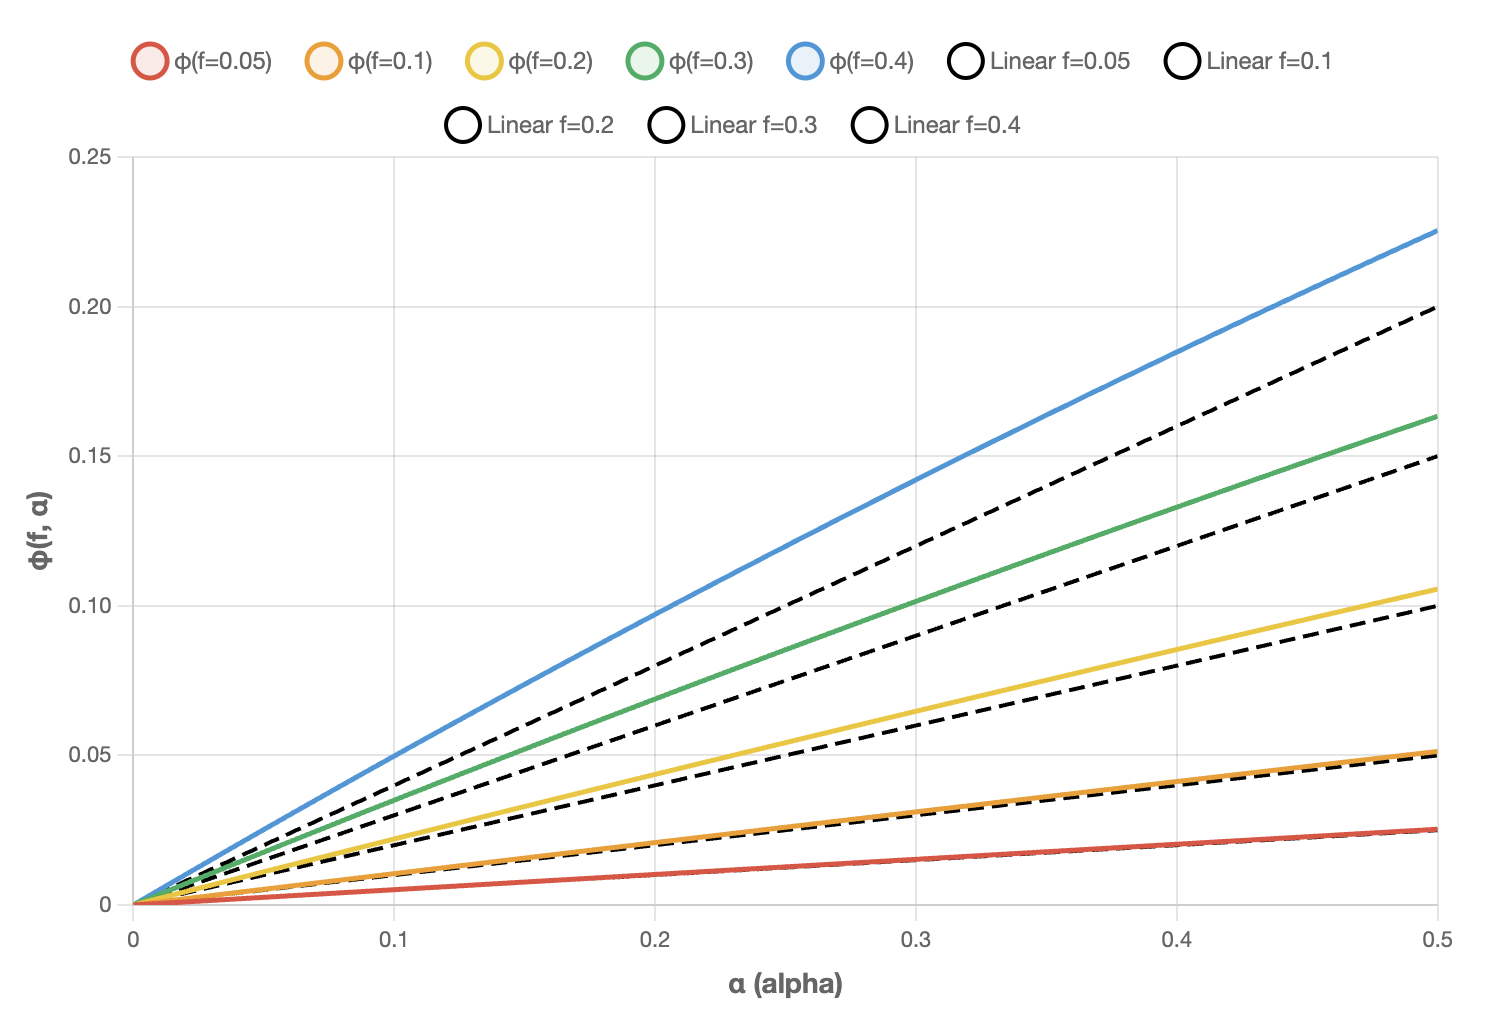
\includegraphics[width=0.9\textwidth]{figs/f-parallelism-bias.png}
\caption{Relationship between $f$, node stake, and the probability of winning a slot.}
\label{fig:f-parallelism-bias}
\end{figure}
%}%%%%%%%%%
Figure~\ref{fig:f-parallelism-bias} shows that increasing $f$ advantages the adversary by raising its chance to win a slot beyond its stake proportion. This effect is stronger when adversarial stake is concentrated in a single entity rather than split across identities.


We choose this method for its simplicity; the resulting overestimation of adversarial capability is acceptable for our purposes. Future work will reduce this bias with an alternative parallelism mechanism.

%\vspace{-.3cm}

\subsection{ILP vs. Global Heuristic}
%\ignore{%%%%%%%%%%%
\begin{figure}[htbp!]
\subfloat[ILP-based optimization]{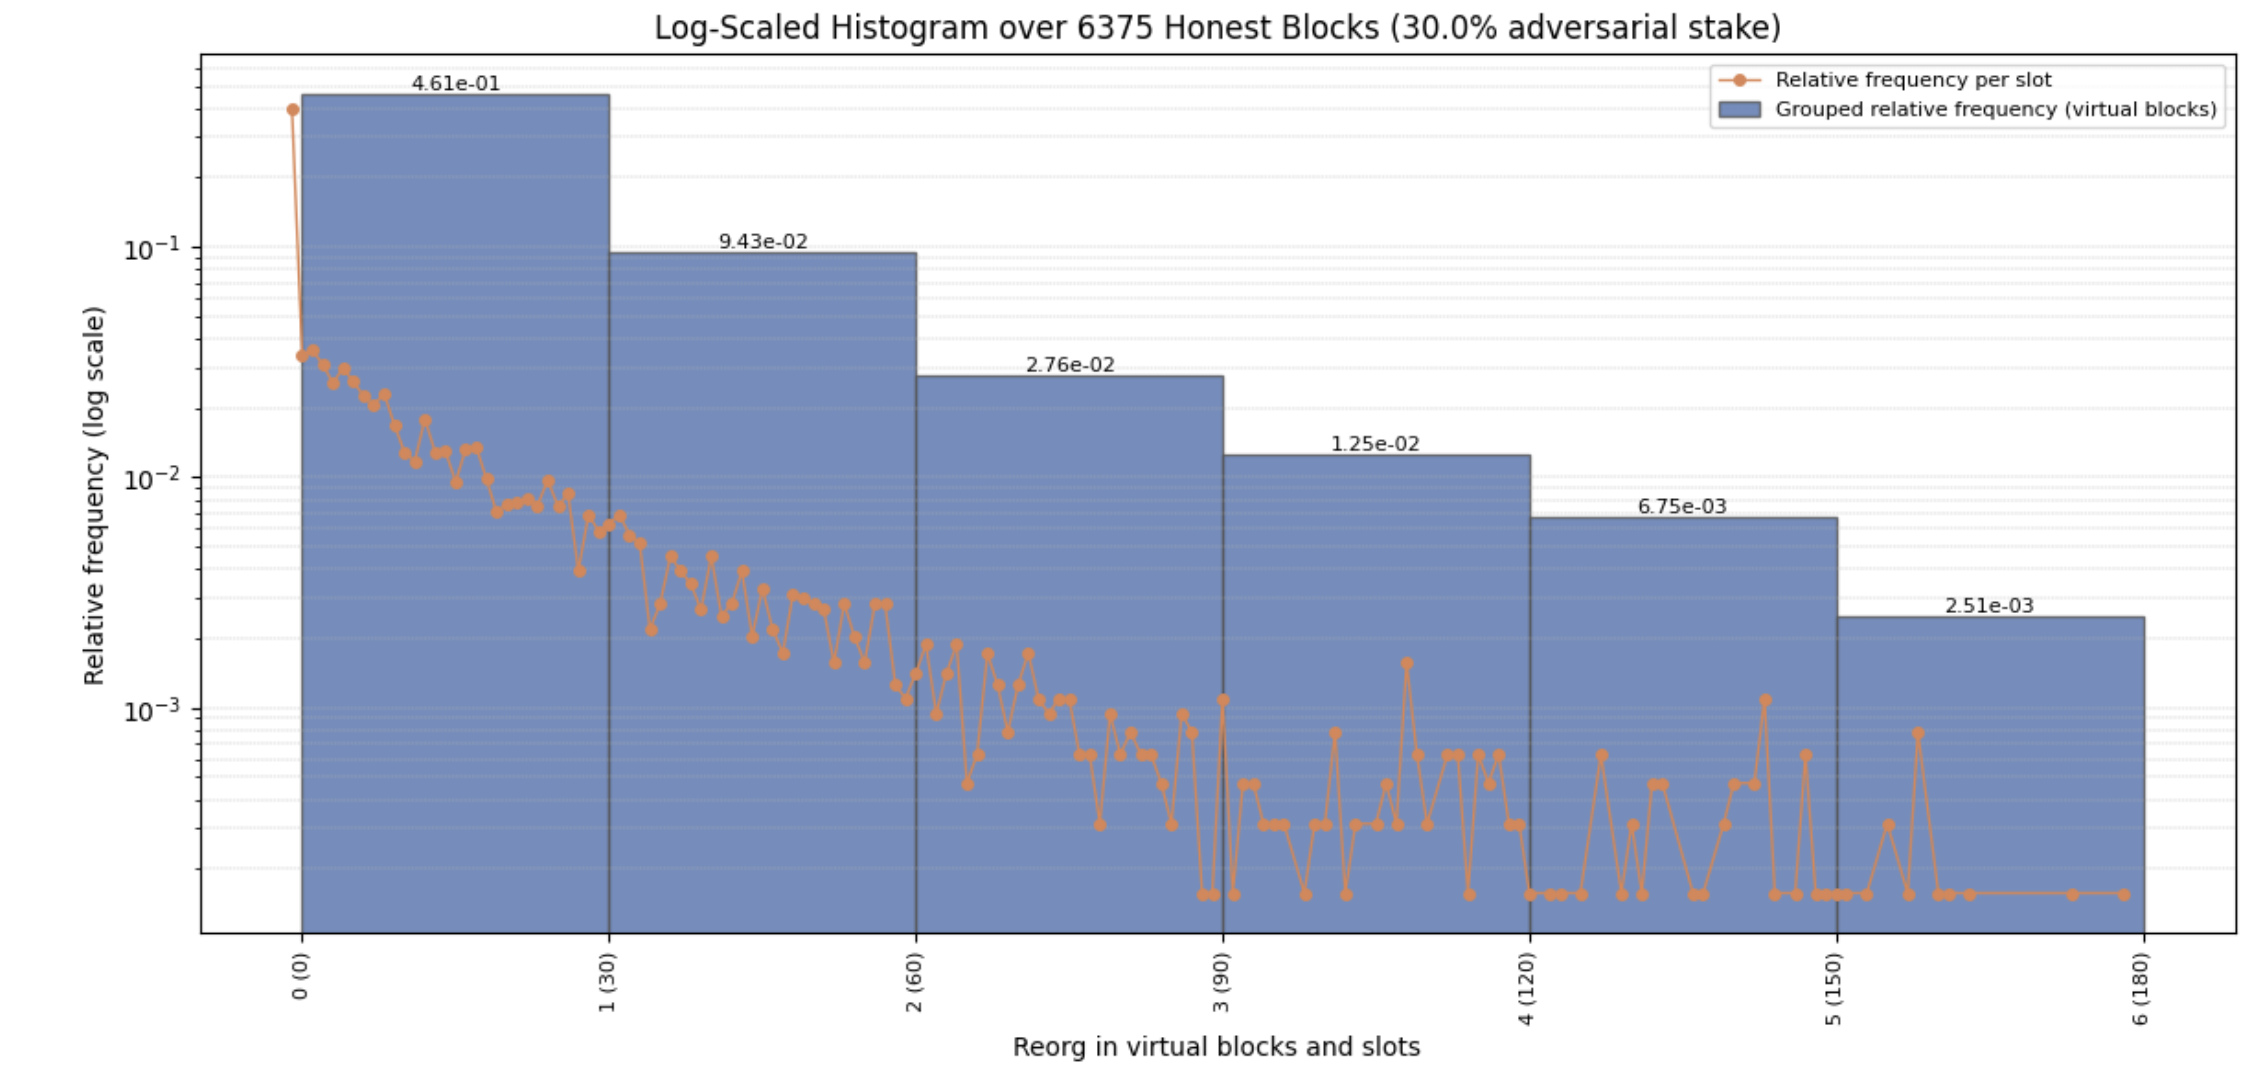
\includegraphics[width=\textwidth/2]{figs/ILP.png}}
\subfloat[Global heuristic optimization]{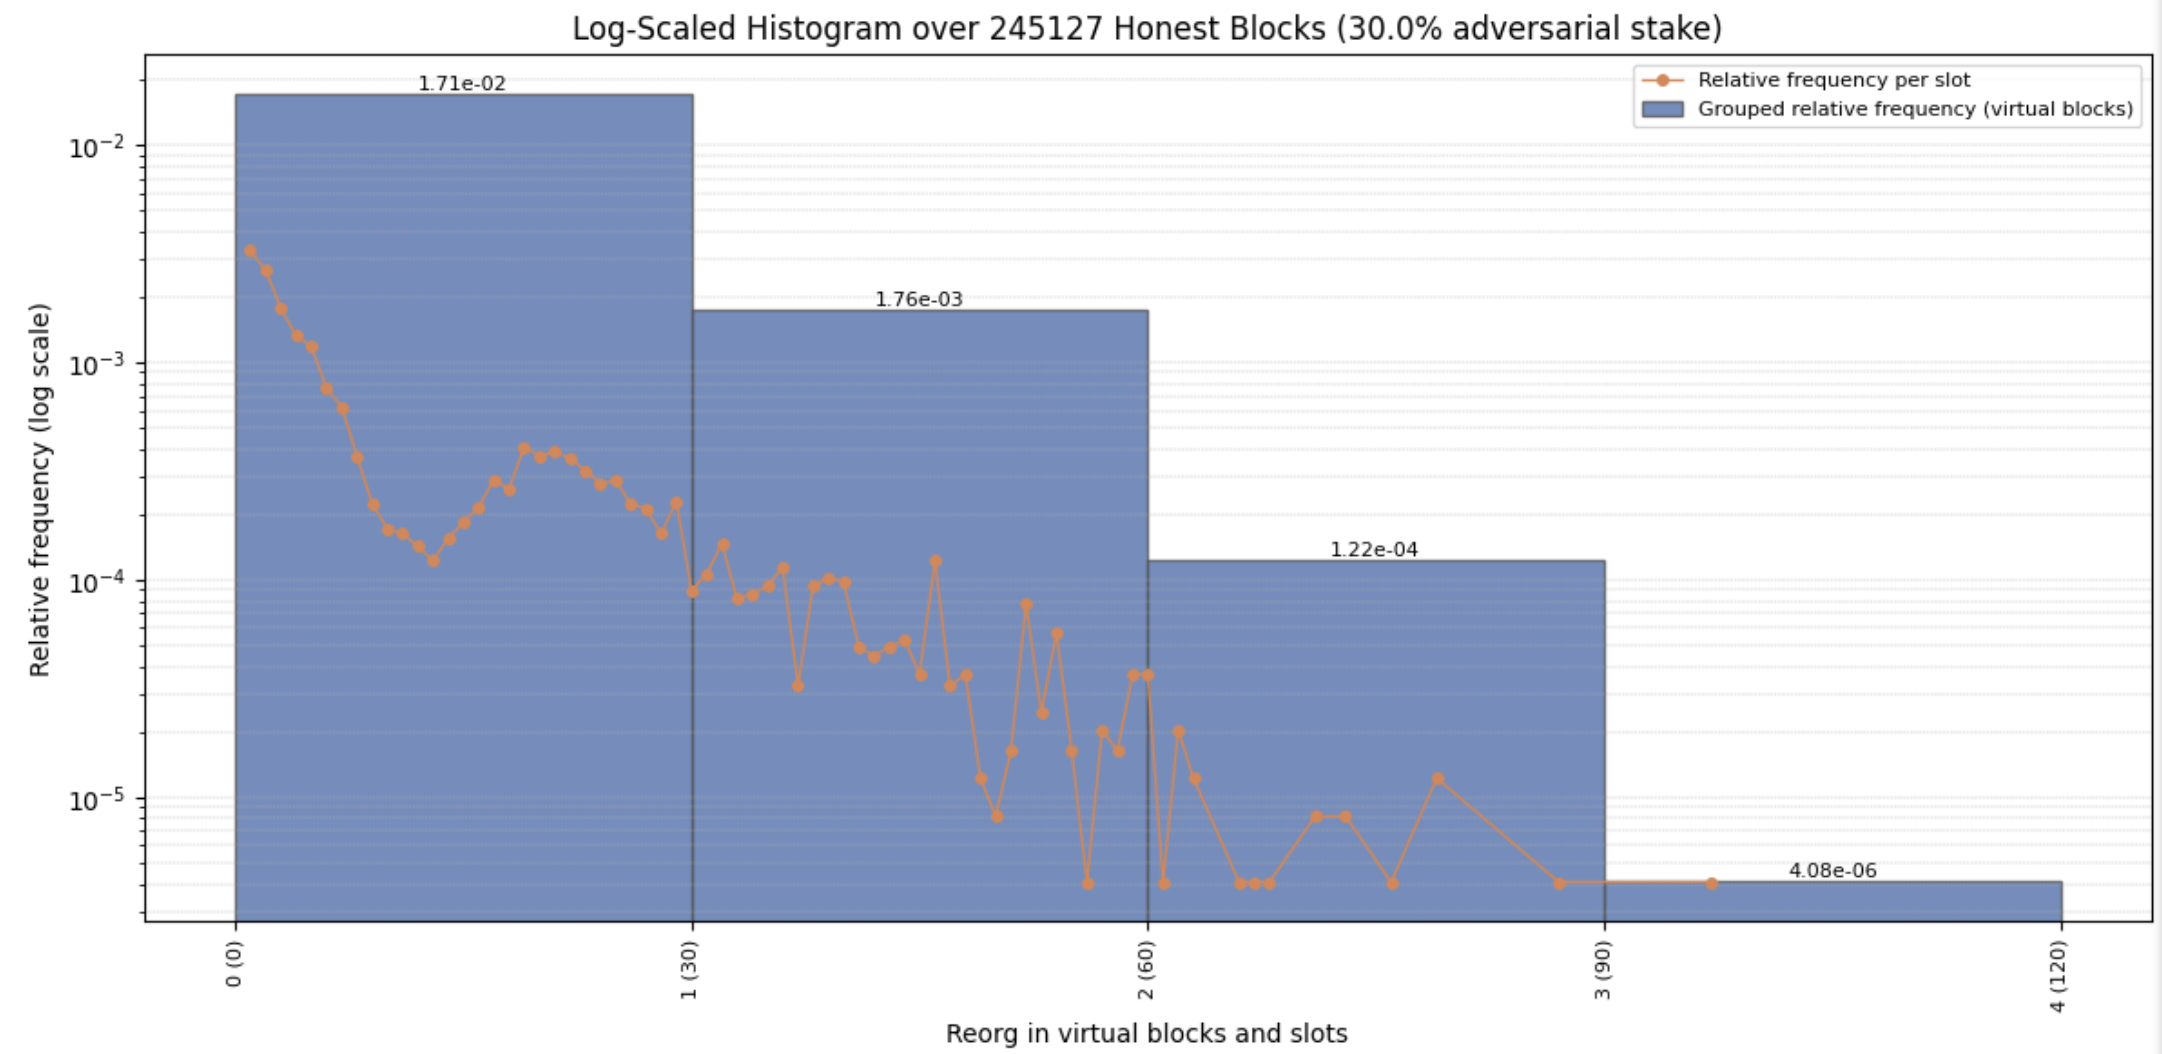
\includegraphics[width=\textwidth/2]{figs/Heuristic.png}}
\caption{Comparison of adversary optimization strategies: ILP-based vs. global heuristic.}
\label{fig:optimization}
\end{figure}
%}%%%%%%%%%%

ILP-based optimization (exhaustive local within the window) yields rarer, longer reorgs but is computationally expensive. The global heuristic scales to many more attacks but produces shorter reorgs on average, consistent with its weaker optimization power (Fig.~\ref{fig:optimization}).


%\ignore{%%%%%%%
\begin{figure}[htbp!]
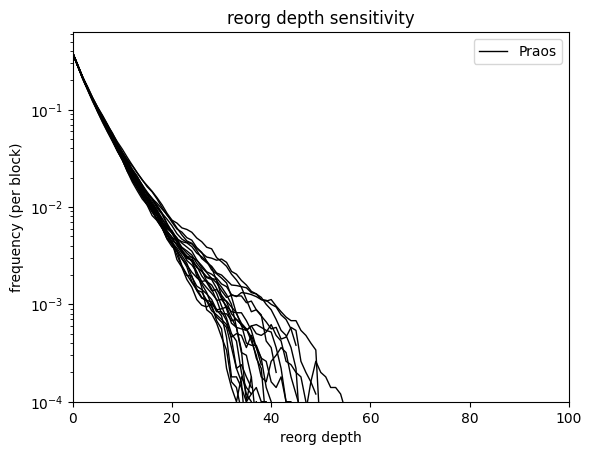
\includegraphics[width=0.7\textwidth]{figs/Praos.png}
\caption{Reorg depth sensitivity of the Ouroboros Praos with $f=0.05$. Black lines present individual chain reorgs depth.}
\label{fig:praos}
\end{figure}
%}%%%%%%%%%

%\vspace{-.3cm}

\subsection{Parallelism vs. Reorg Length}

%\ignore{%%%%%%%
\begin{figure}[htbp!]
\subfloat[5x parallelization, $f=0.25$]{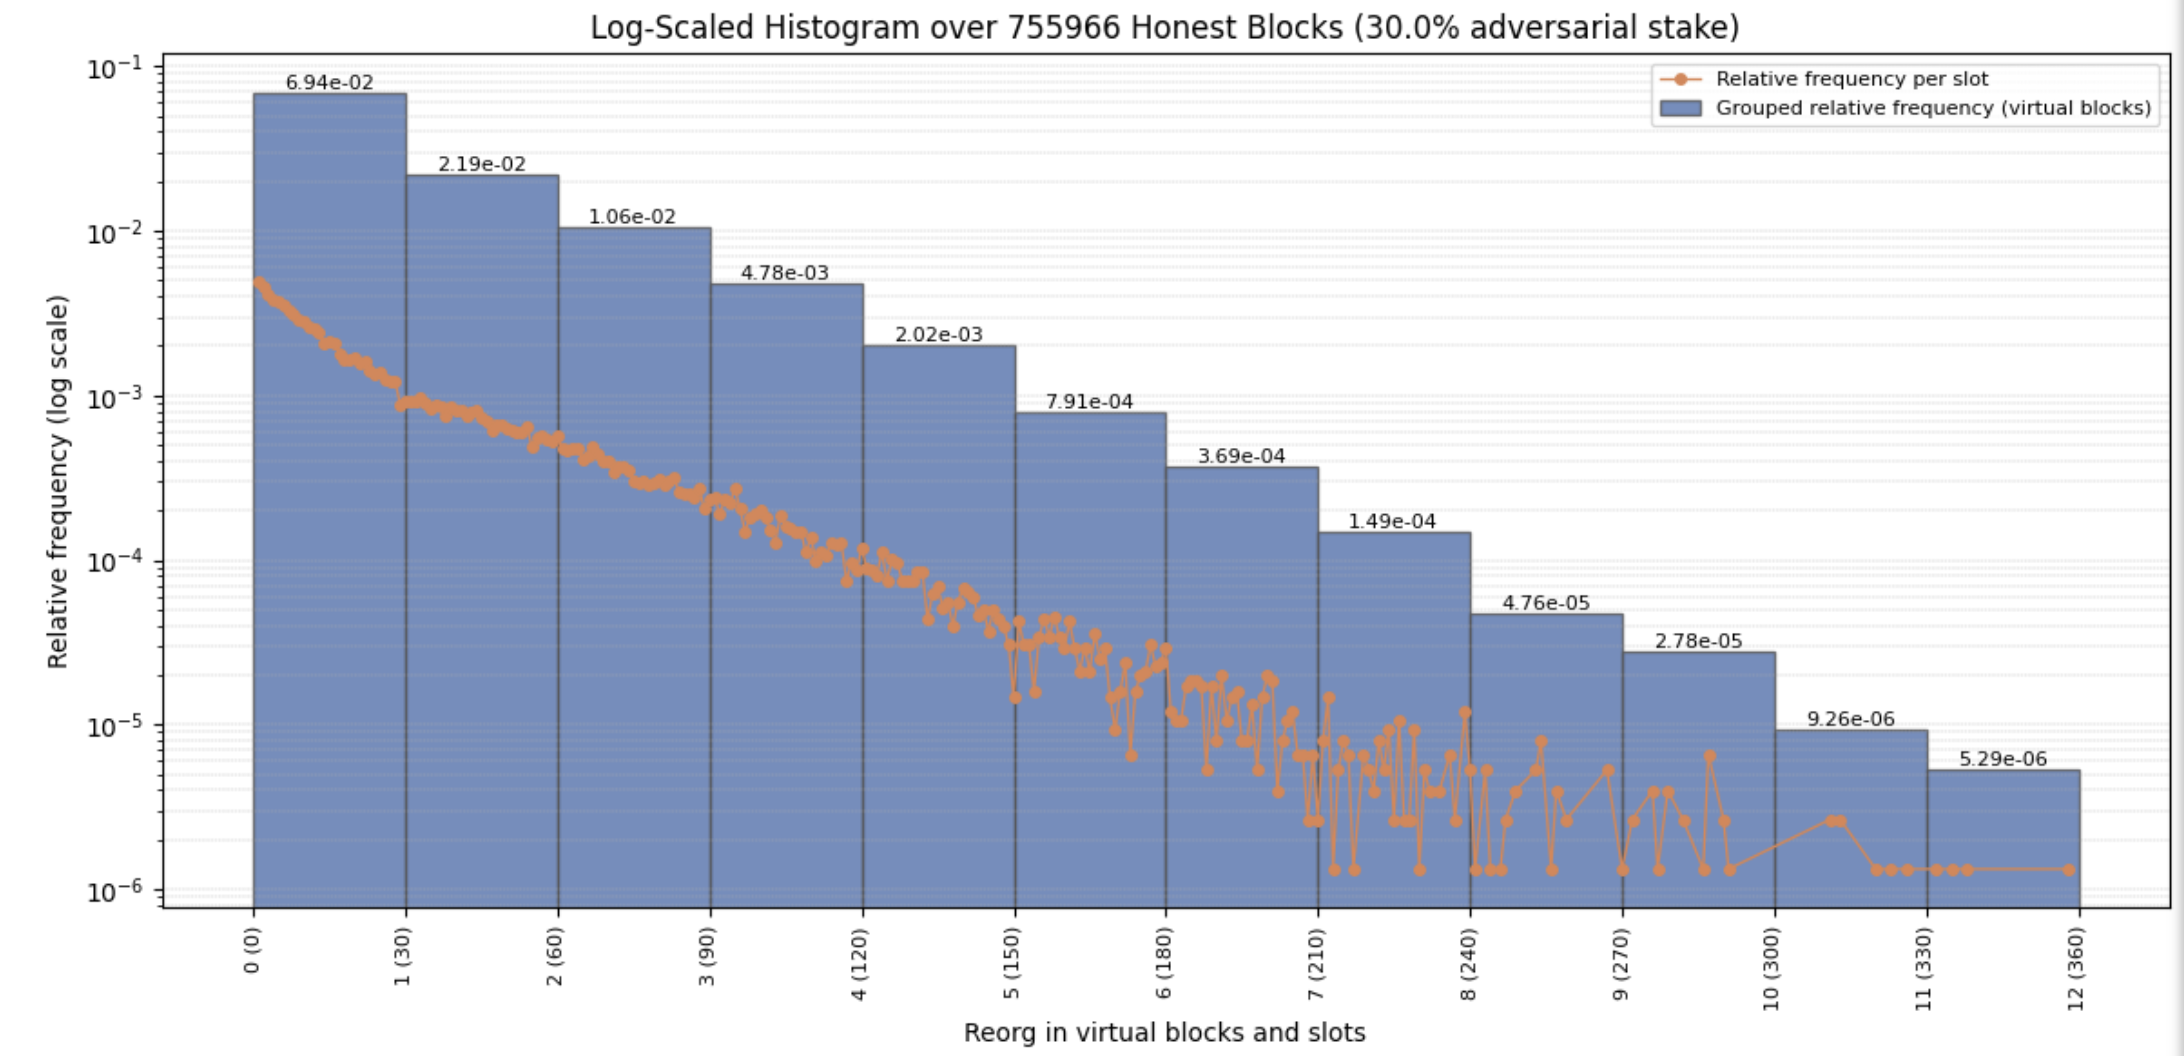
\includegraphics[width=\textwidth/2]{figs/f-0.25.png}}
\subfloat[6x parallelization, $f=0.30$]{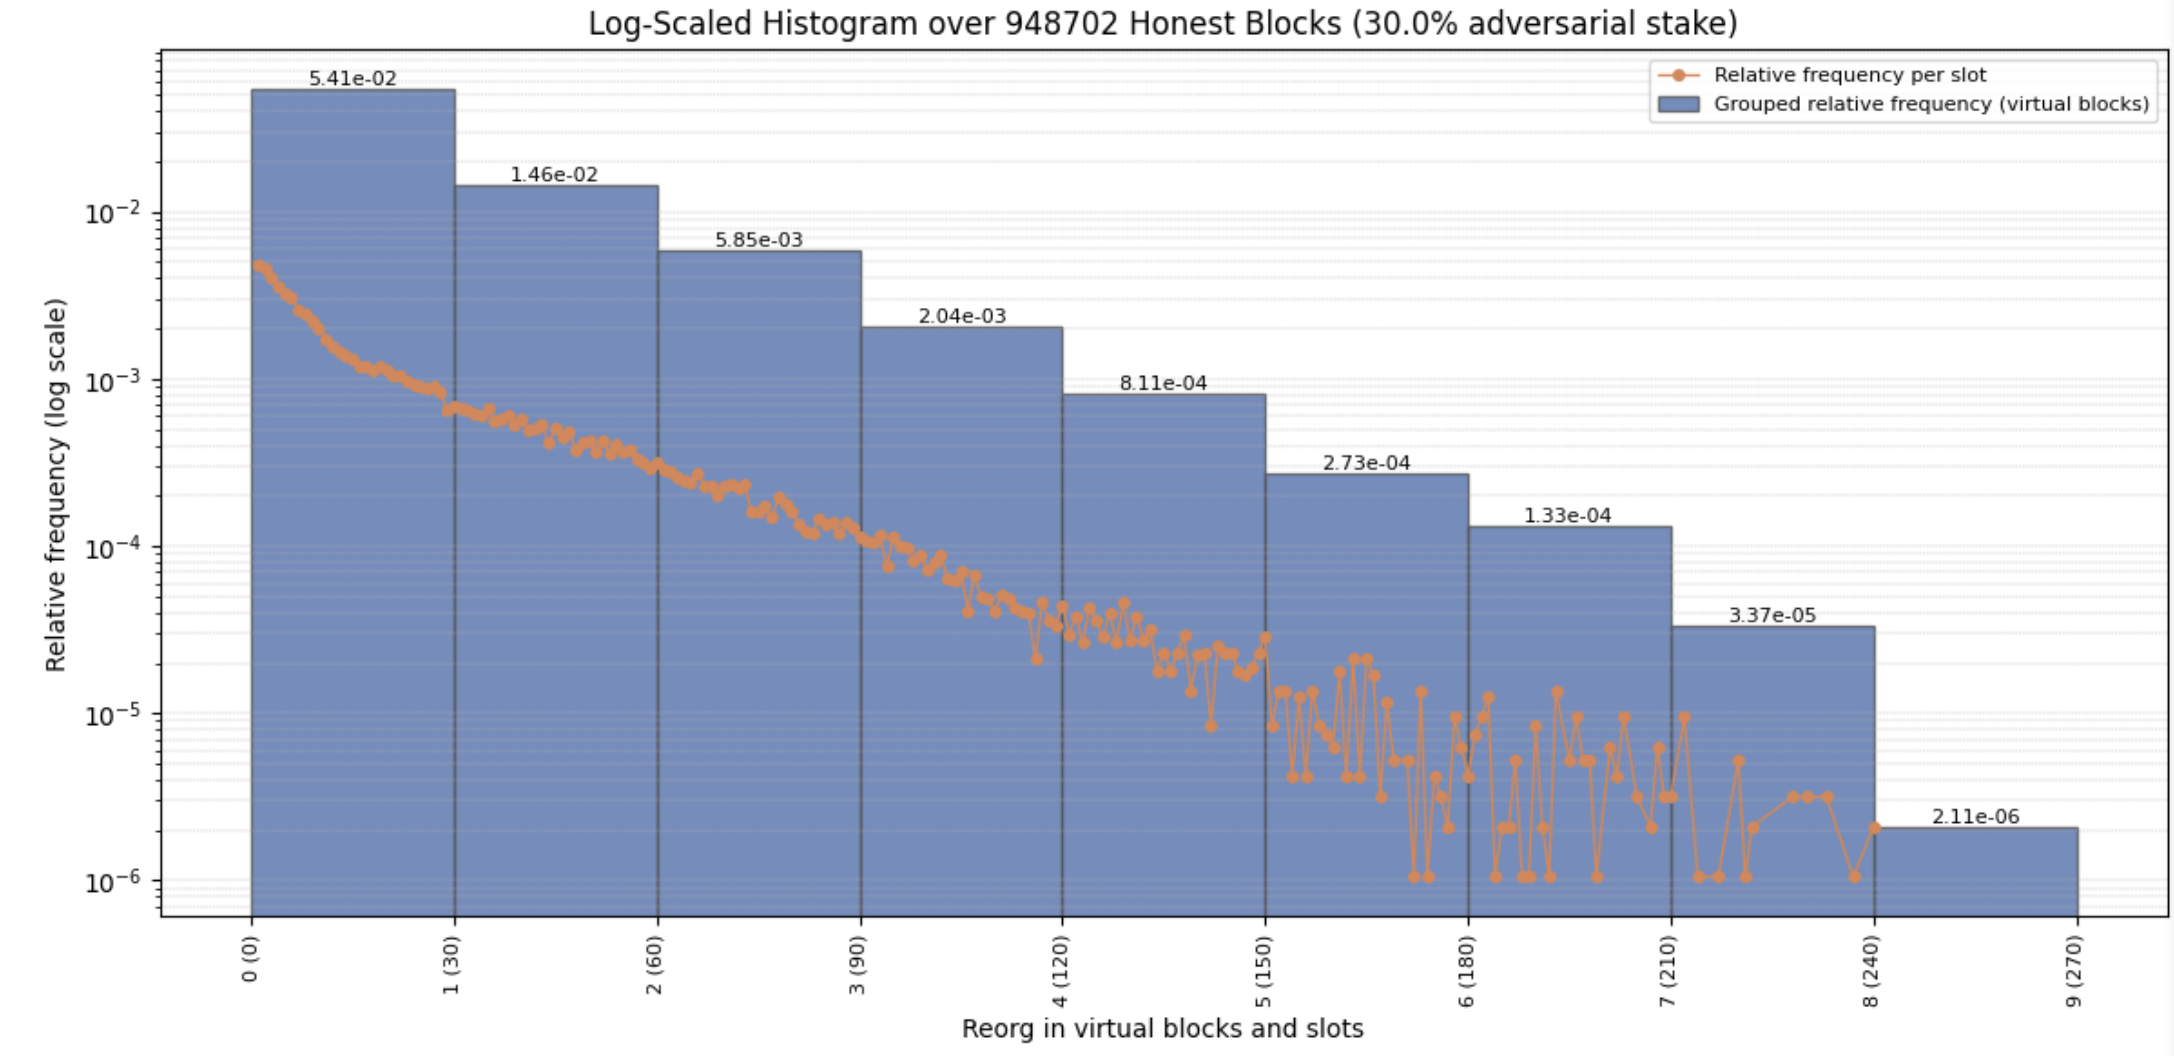
\includegraphics[width=\textwidth/2]{figs/f-0.30.png}}\\
\subfloat[7x parallelization, $f=0.35$]{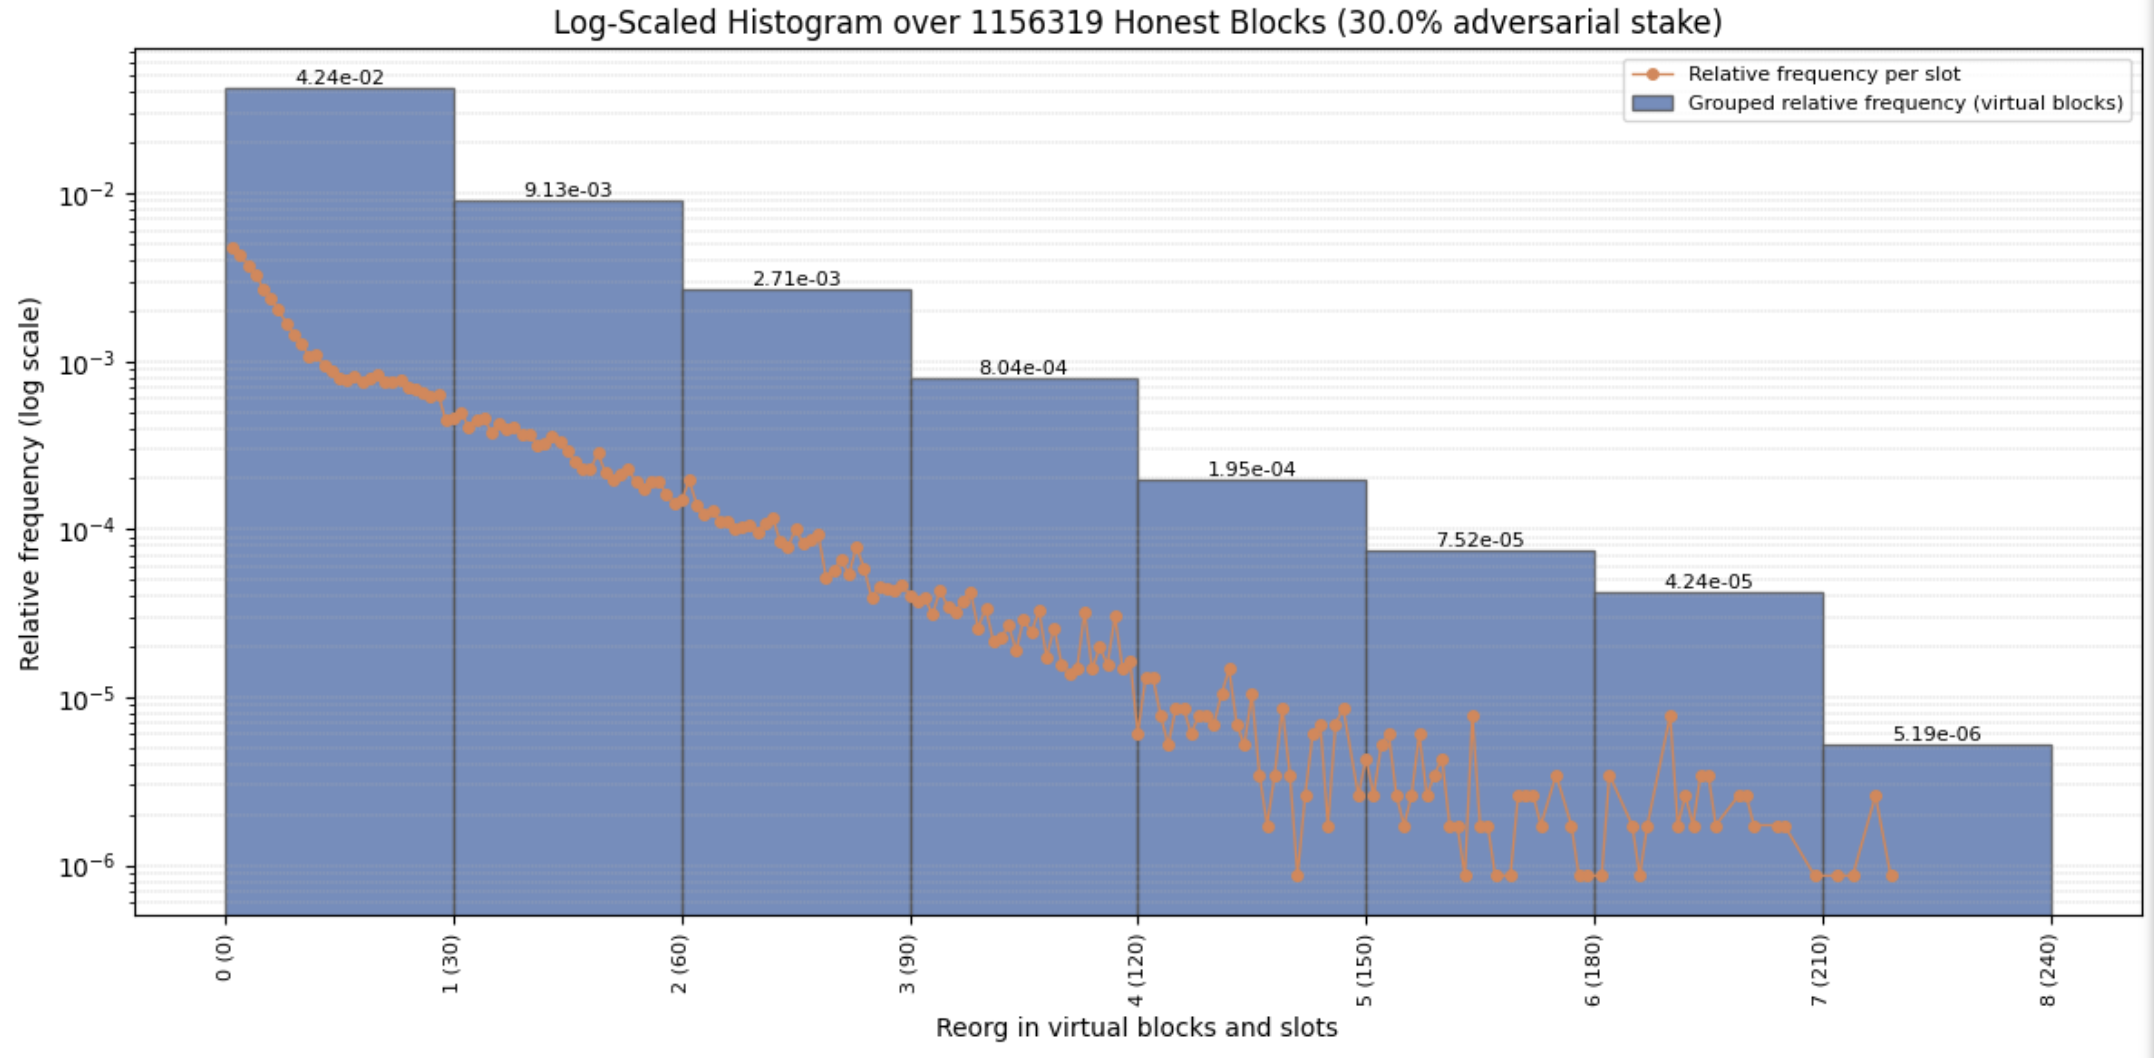
\includegraphics[width=\textwidth/2]{figs/f-0.35.png}}
\subfloat[8x parallelization, $f=0.40$]{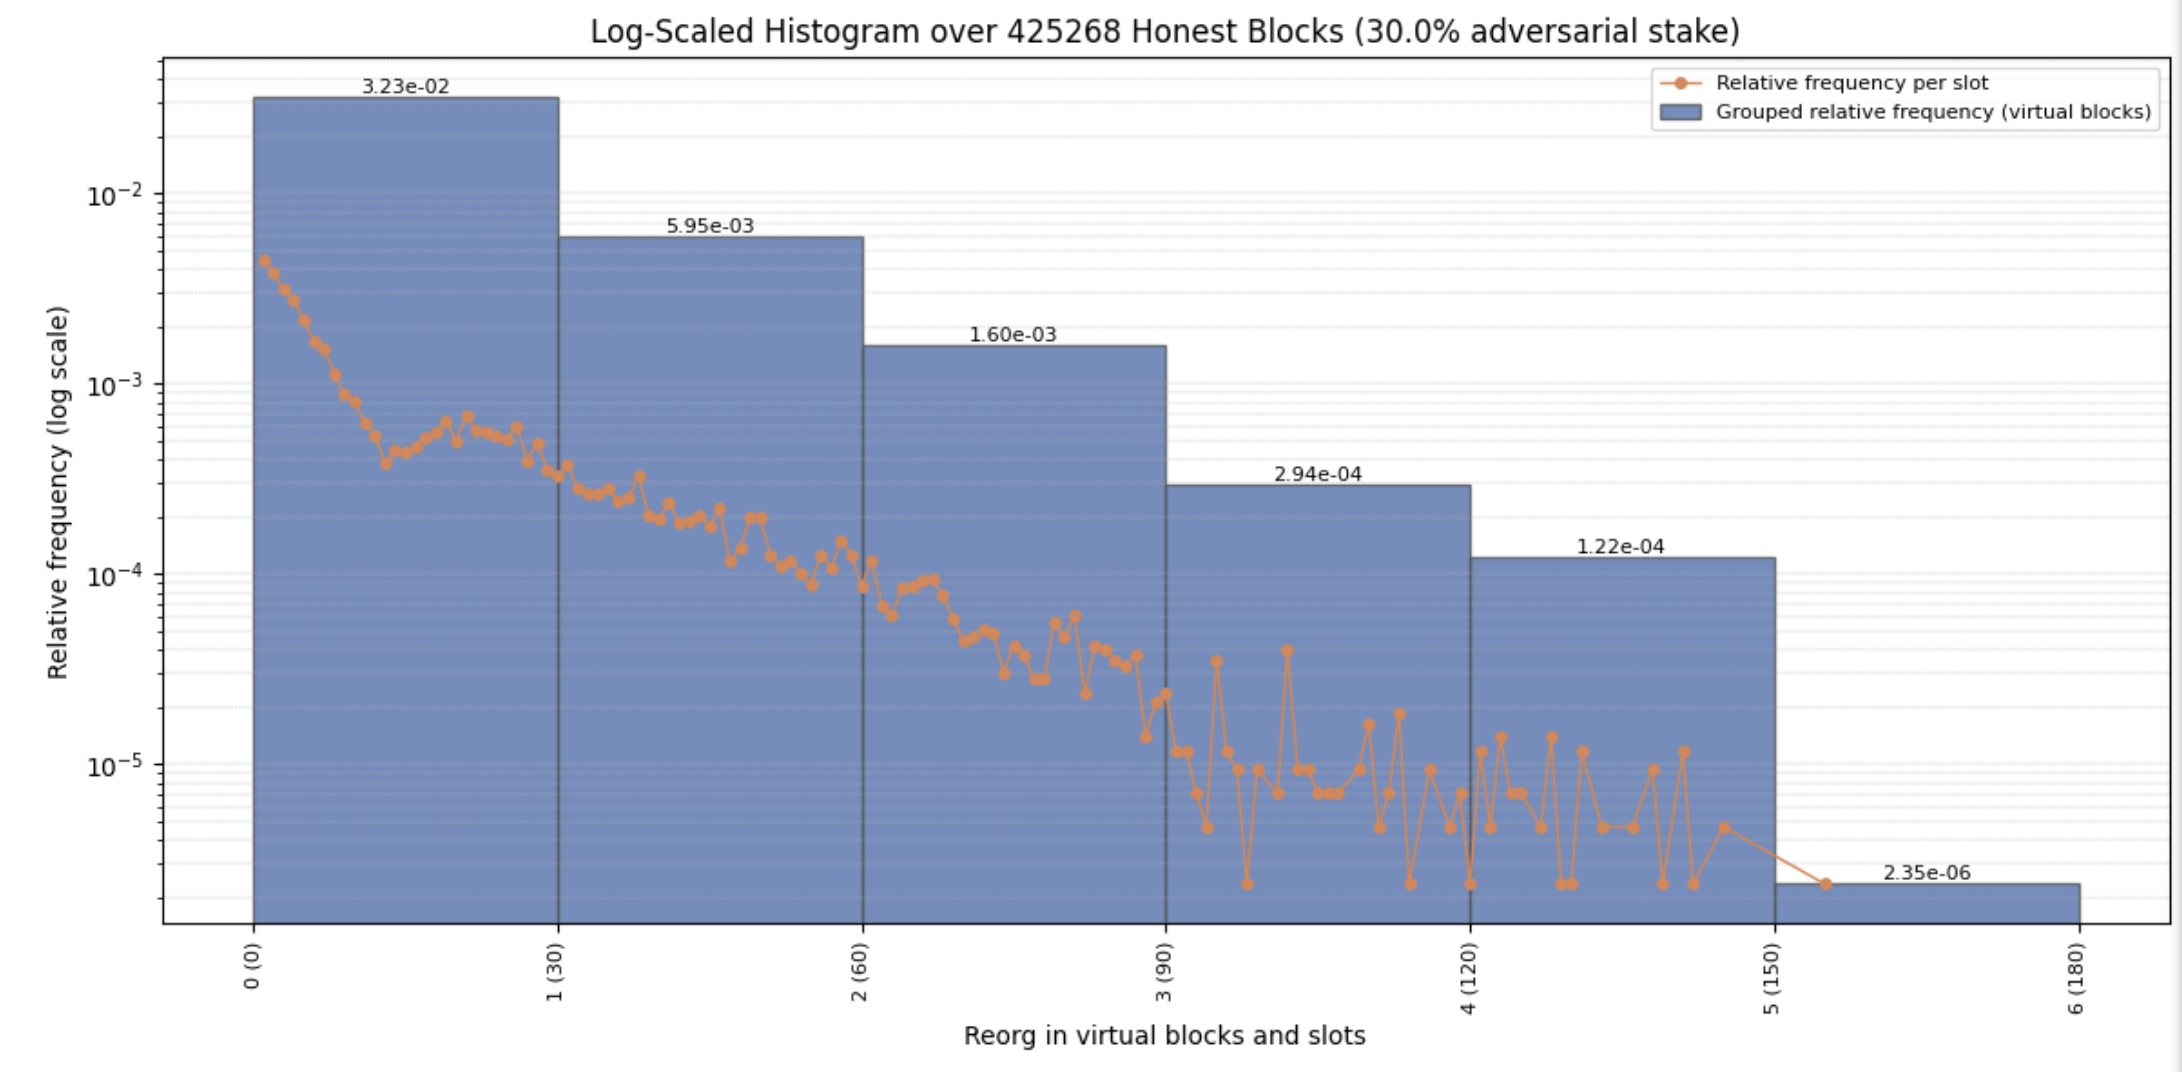
\includegraphics[width=\textwidth/2]{figs/f-0.40.png}}\\
\subfloat[10x parallelization, $f=0.50$]{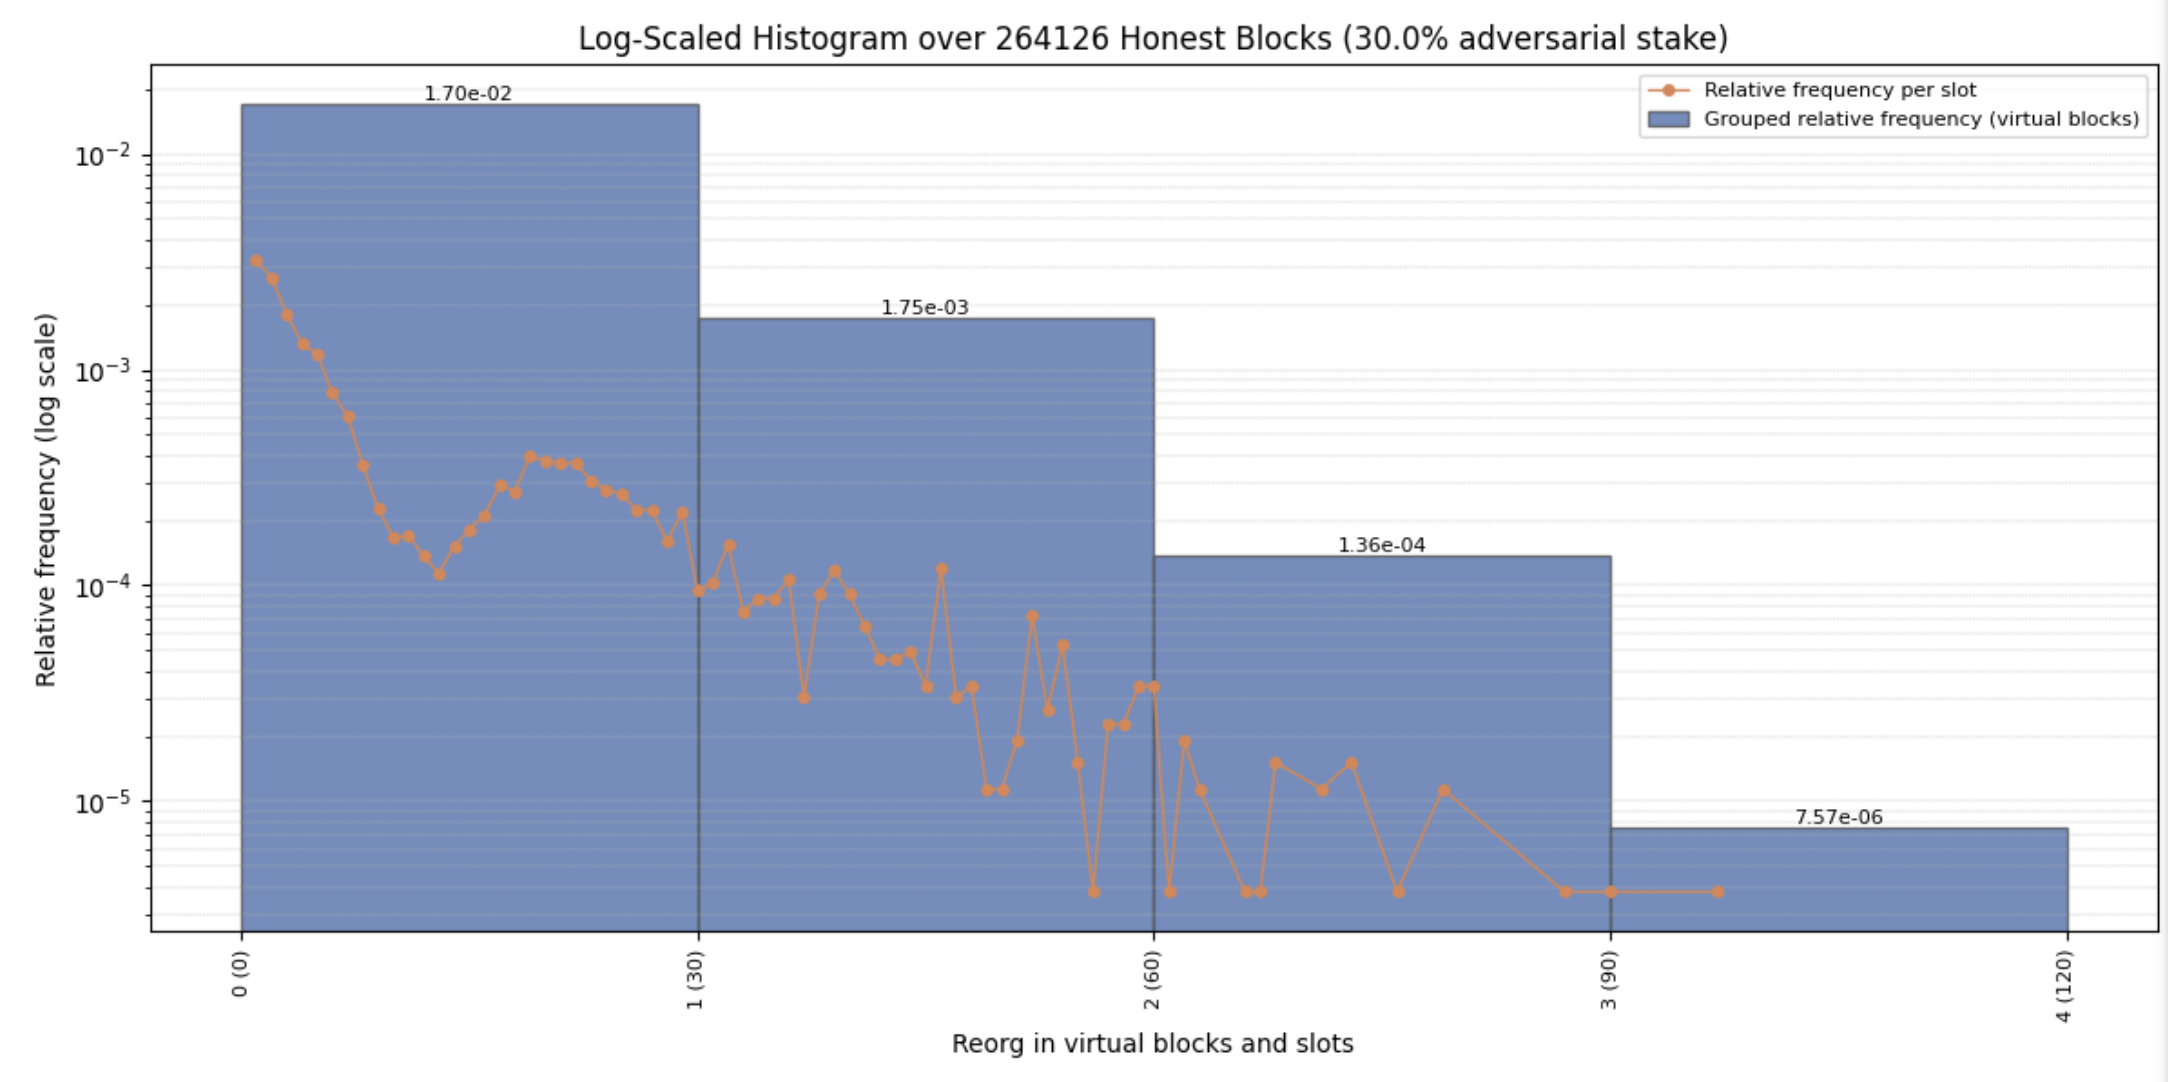
\includegraphics[width=\textwidth]{figs/f-0.50.png}}
\caption{Impact of parallelization level on reorg depth for \ProjBase{} with 30\% adversarial stake.}
\label{fig:parallelization}
\end{figure}
%}%%%%%%%
Empirically, higher parallelism (larger $f$) correlates with shorter reorgs, especially in large-scale heuristic runs that enable more attack attempts (Fig.~\ref{fig:parallelization}). ILP-based local optima can surface rare long reorgs in small samples, but across $f\in\{0.25,0.30,0.35,0.40,0.50\}$ tail depth decreases as $f$ increases, aligning with the “more votes, faster convergence” intuition.

%\subsection{Reorg Distributions vs. Stake and Latency}
%We assess how attacker capability (stake fraction and network control) affects the distribution of reorg depths and times. We vary $\alpha$ from $0.10$ to $0.49$ and test $\Delta$ from $0.2$ s to $2$ s, holding other parameters fixed. For each setting, we simulate long runs (up to $10^6$ slots) to obtain distributions of reorg length and finalization time.

\begin{figure}[htbp!]
\subfloat[30\% of adversarial stake]{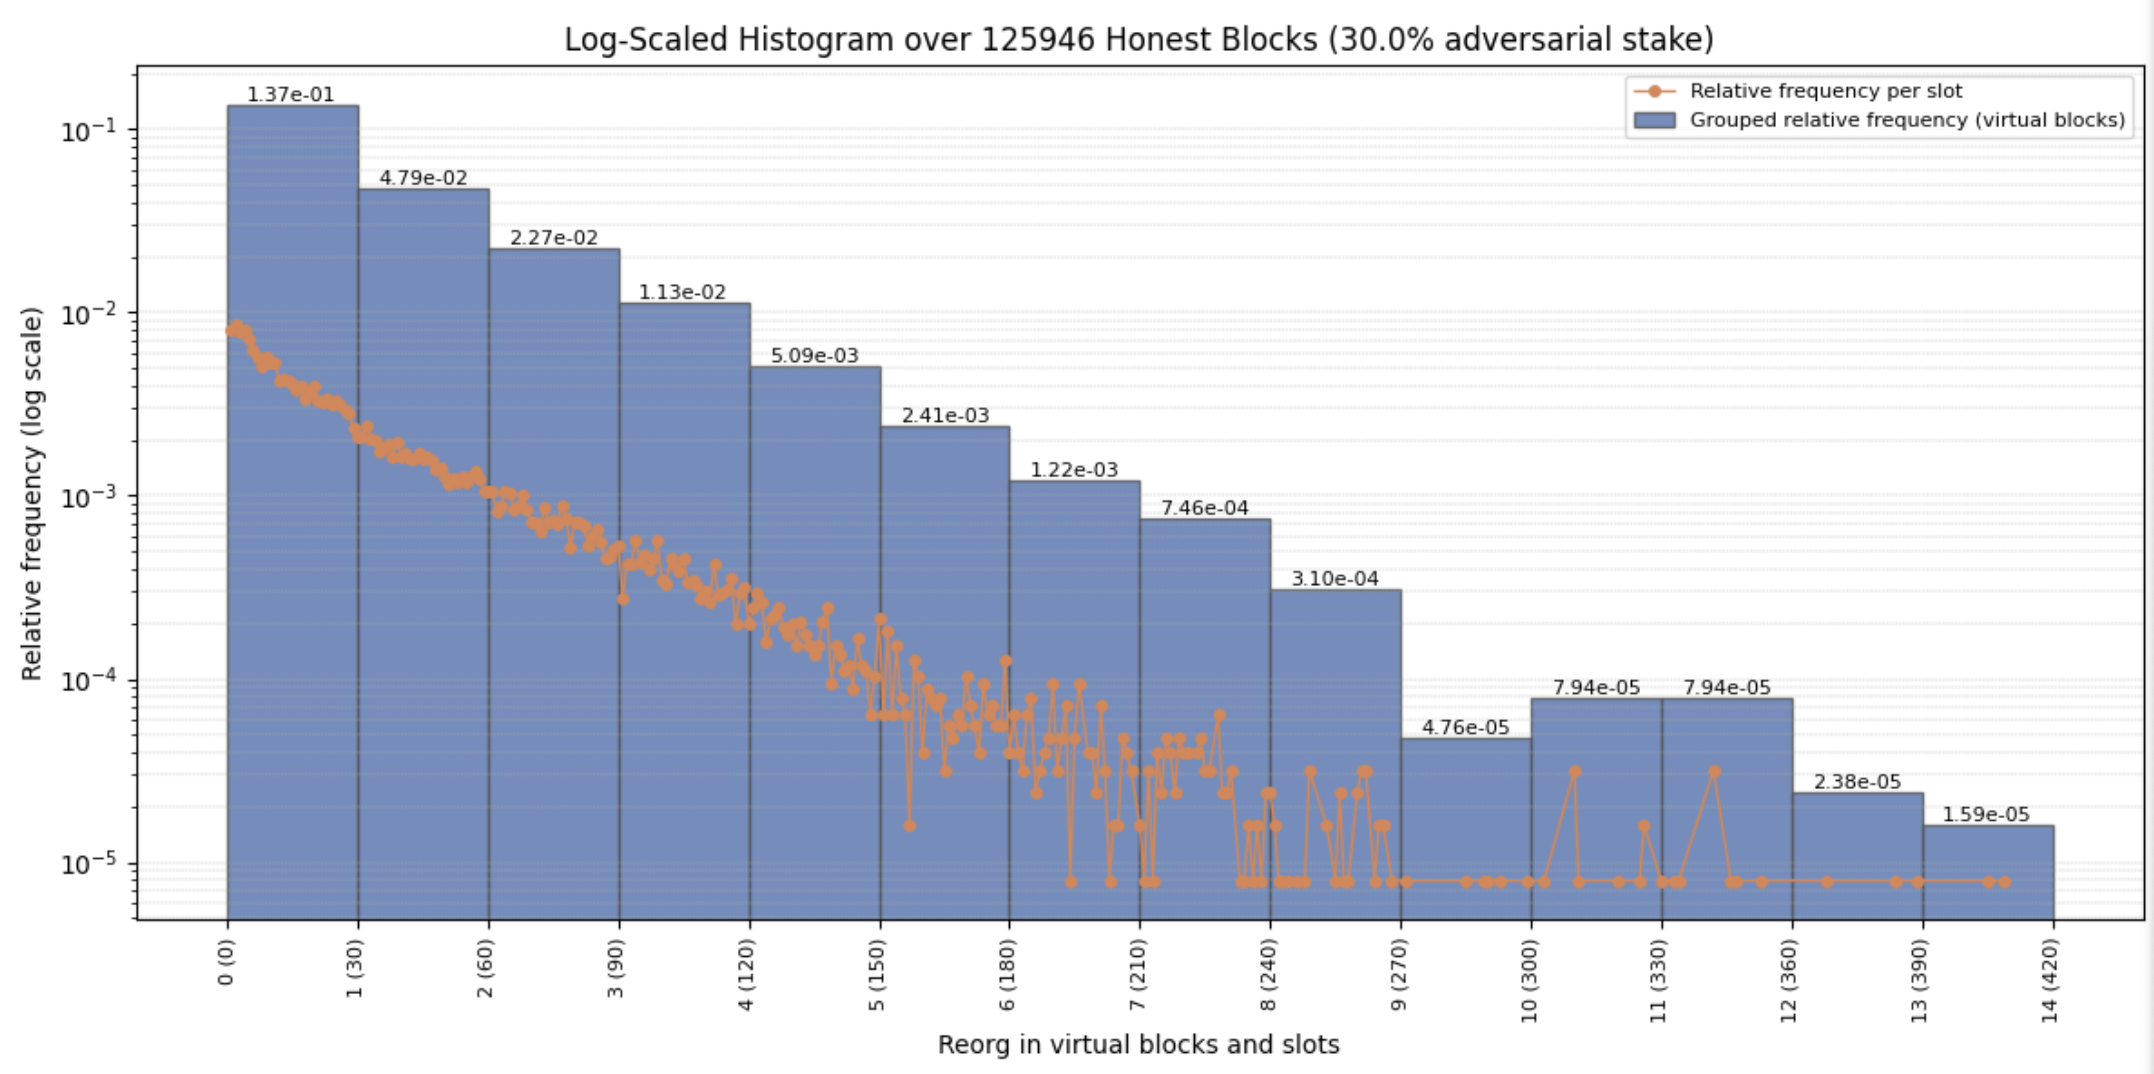
\includegraphics[width=\textwidth/2]{figs/adv-30.png}}
\subfloat[40\% of adversarial stake]{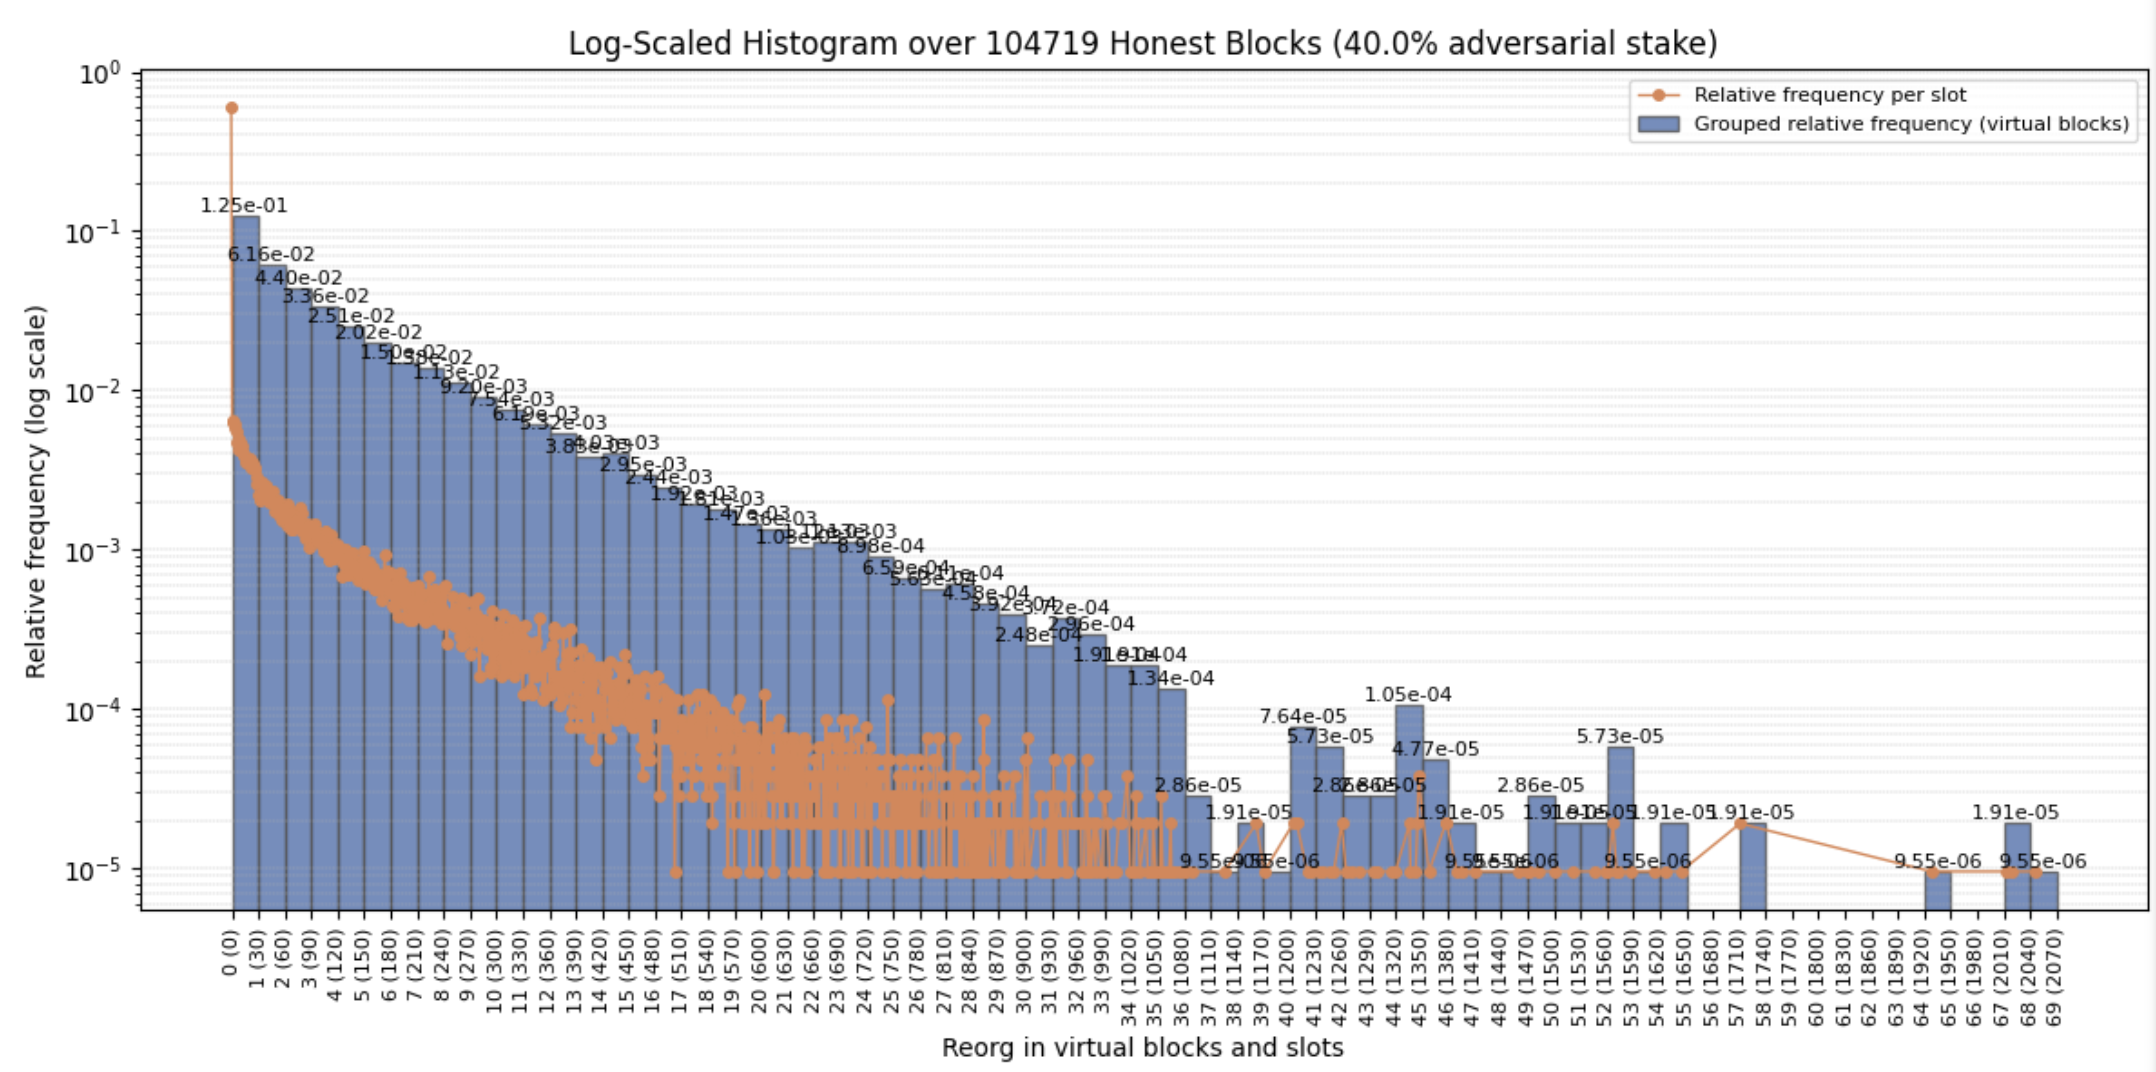
\includegraphics[width=\textwidth/2]{figs/adv-40.png}}\\
\subfloat[45\% of adversarial stake]{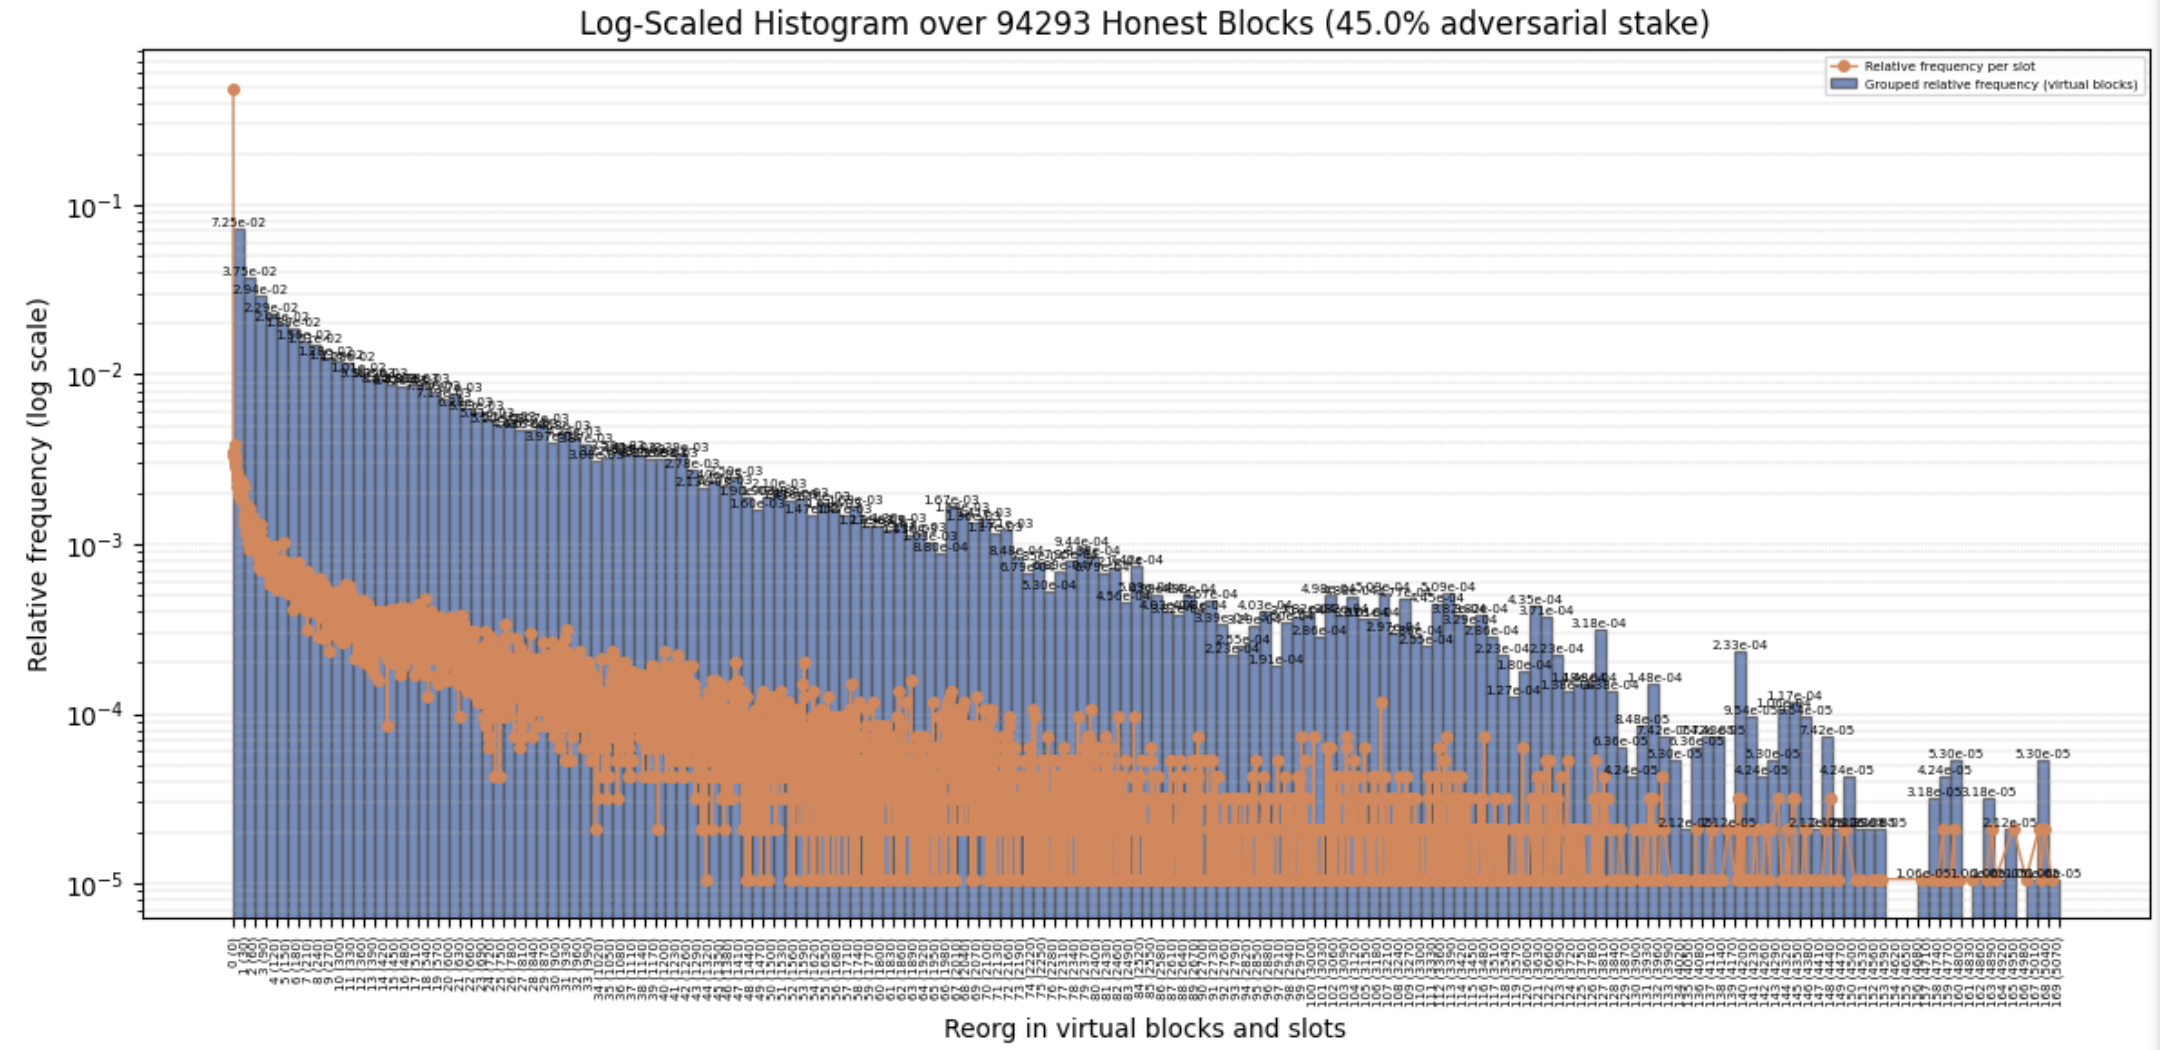
\includegraphics[width=\textwidth/2]{figs/adv-45.png}}
\subfloat[49\% of adversarial stake]{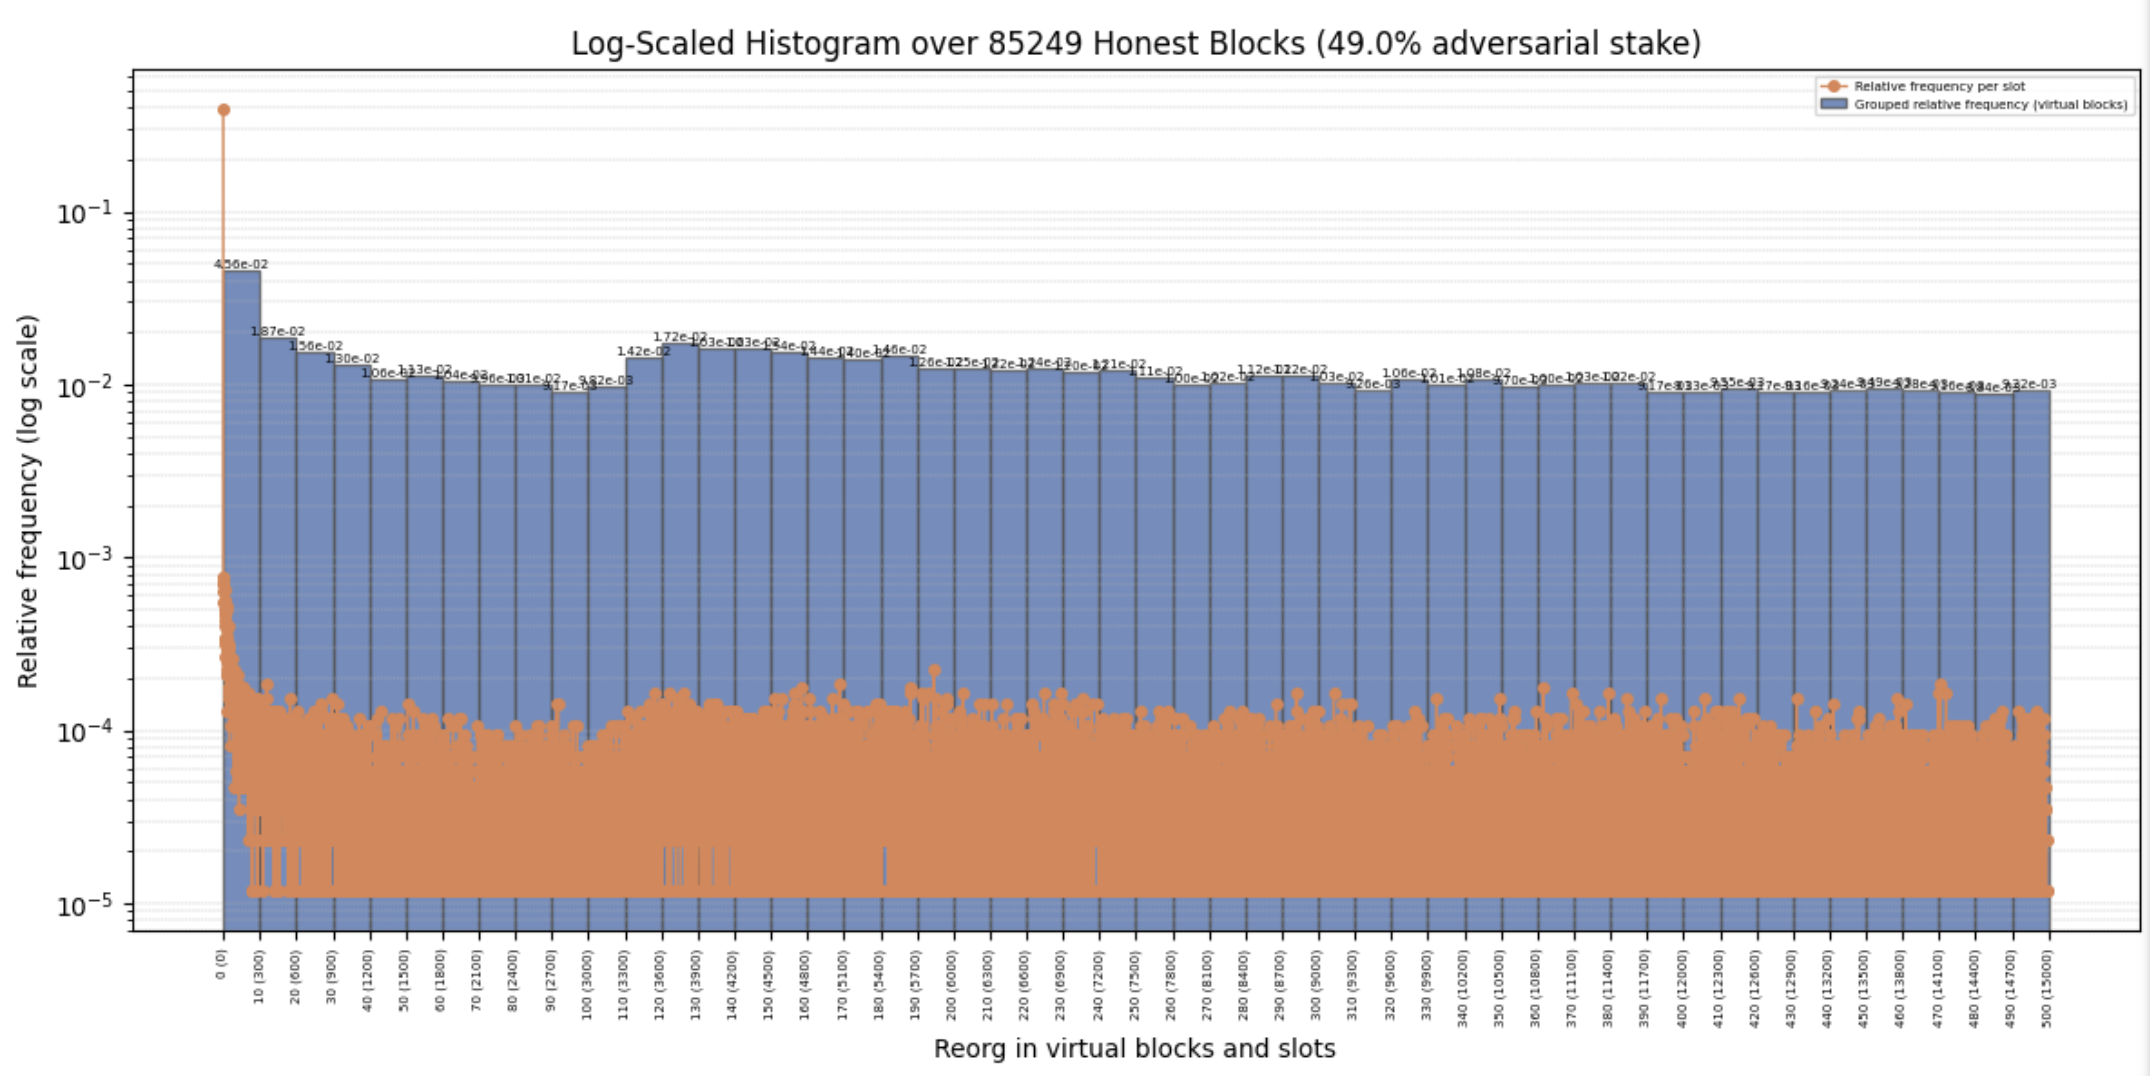
\includegraphics[width=\textwidth/2]{figs/adv-49.png}}\\
\subfloat[51\% of adversarial stake]{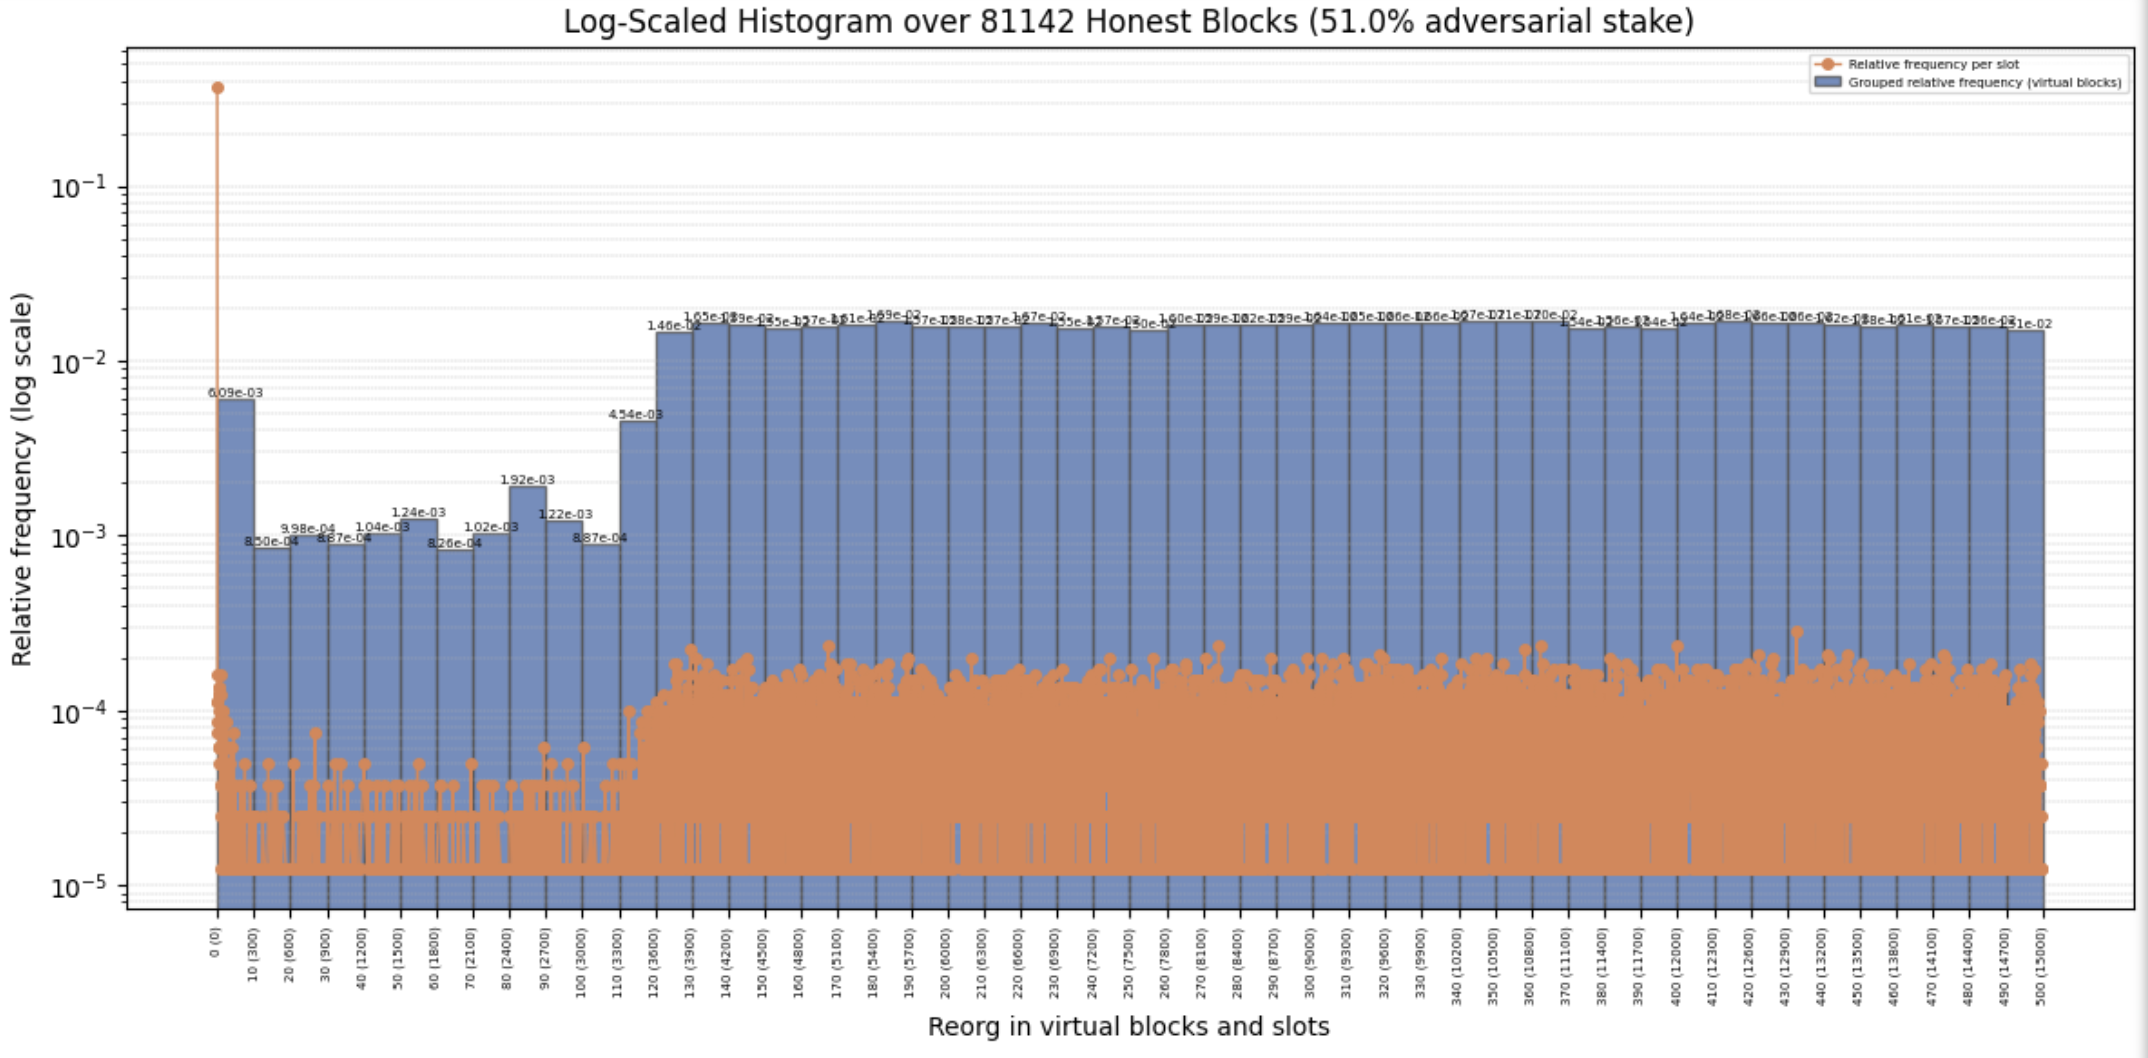
\includegraphics[width=\textwidth/2]{figs/adv-51.png}}
\subfloat[60\% of adversarial stake]{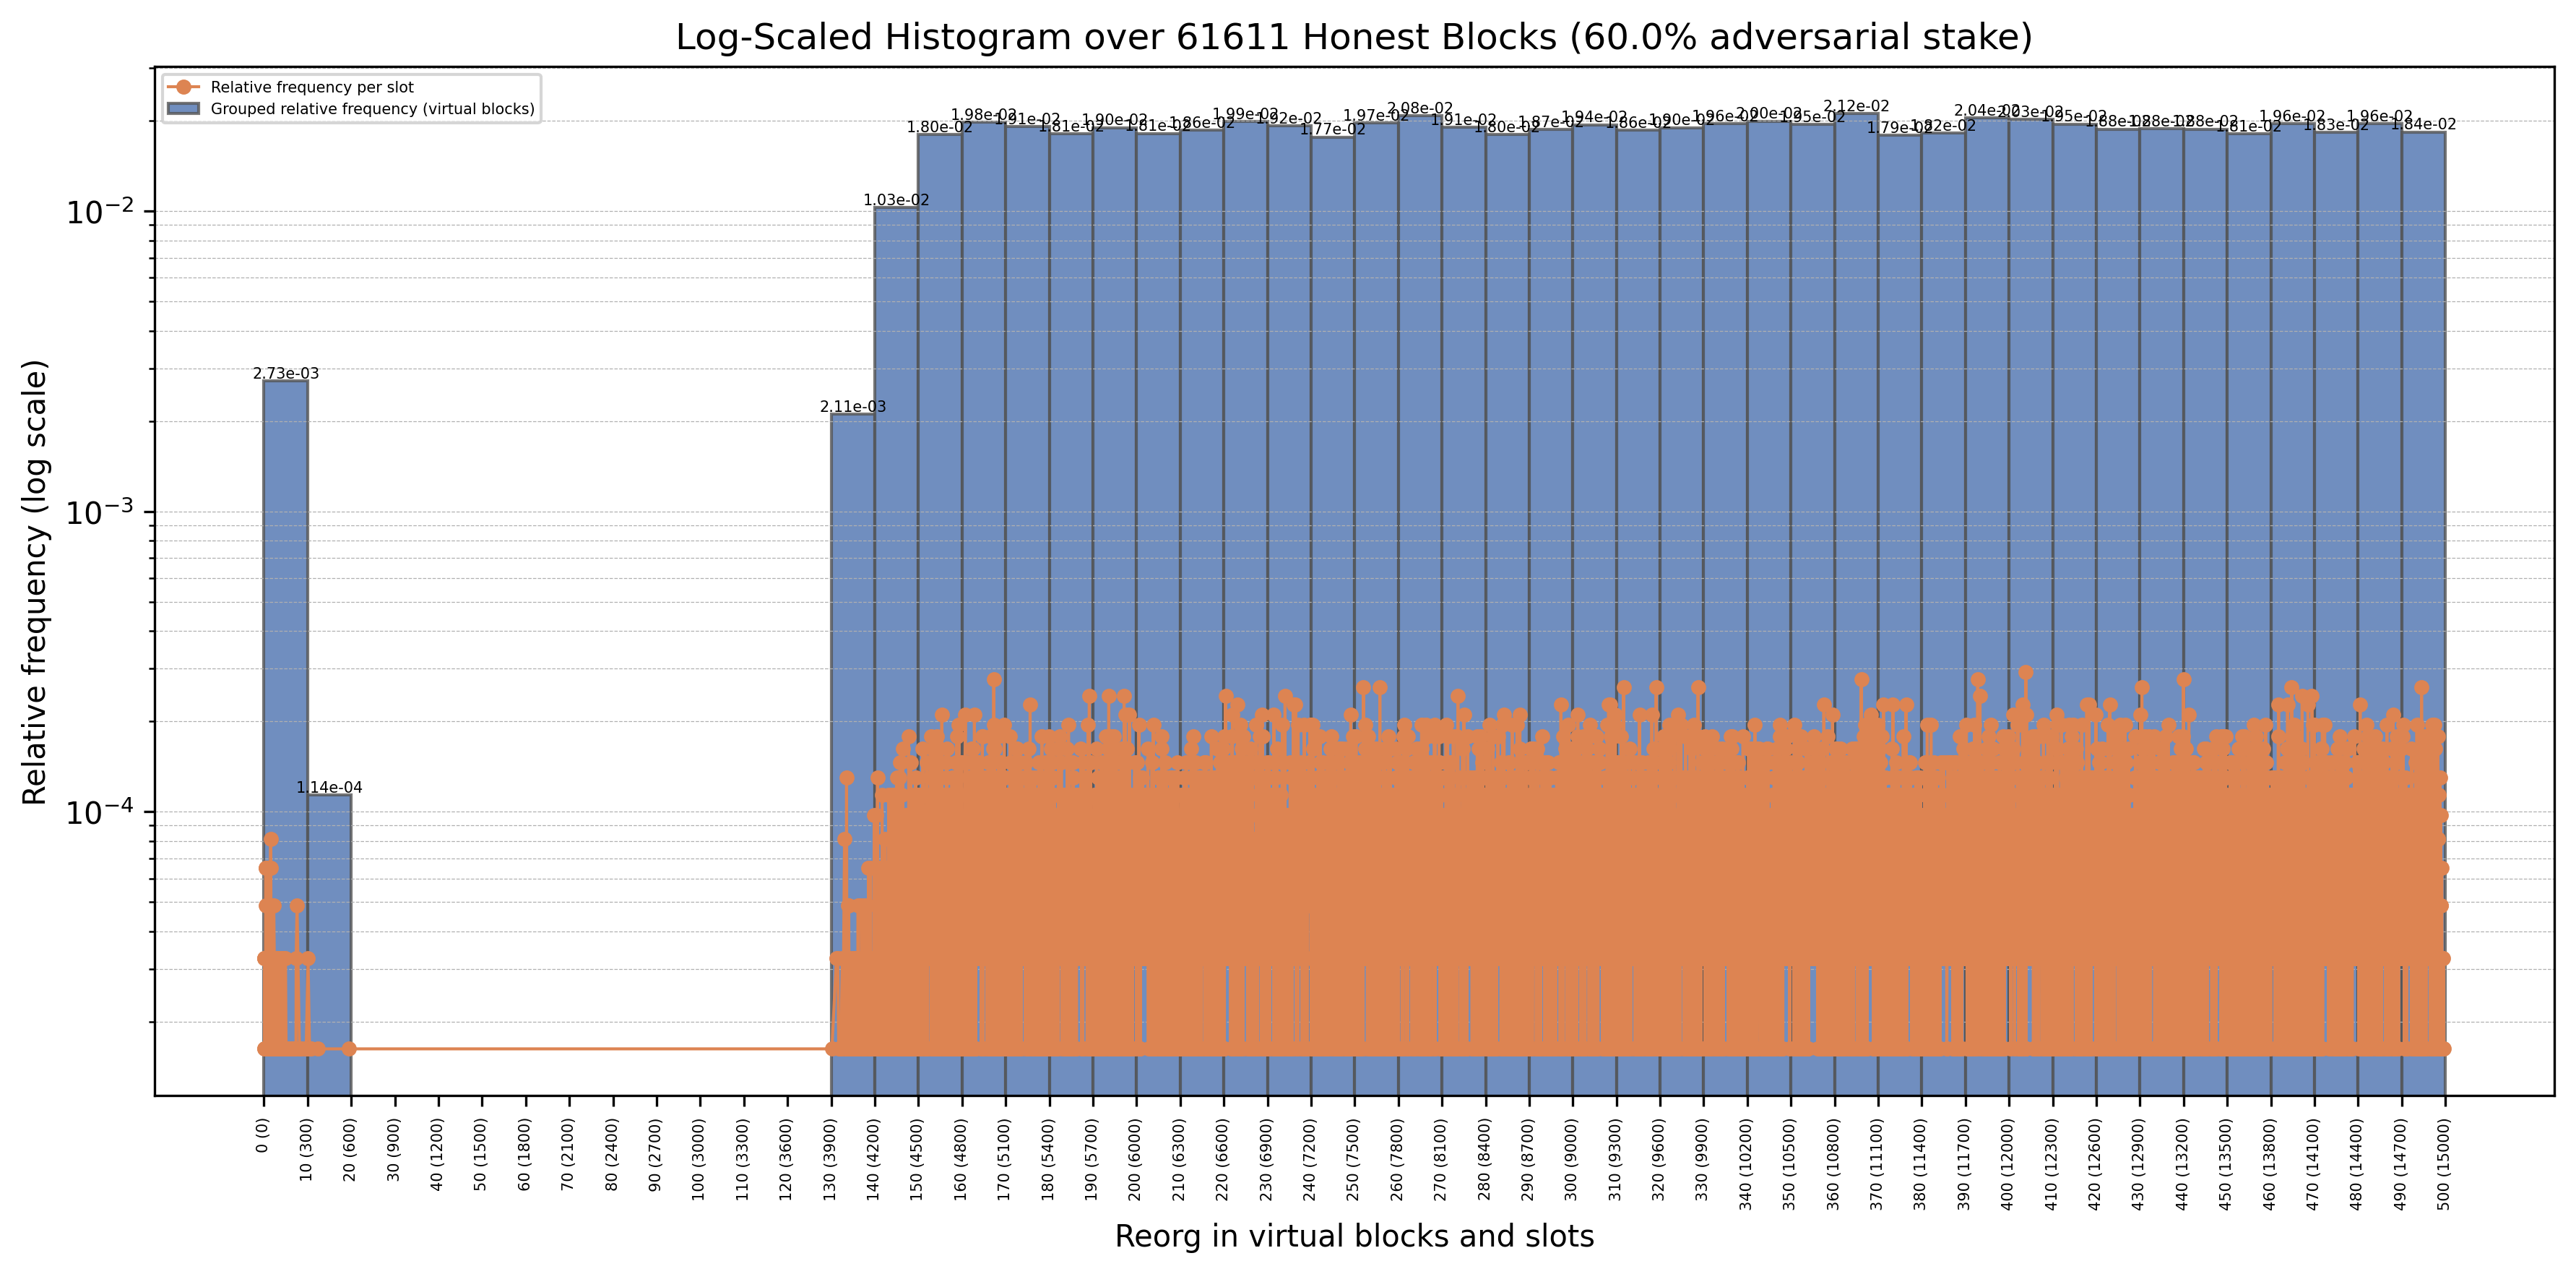
\includegraphics[width=\textwidth/2]{figs/adv-60.png}}
\caption{Impact of the adversarial stake delay on the reorg depth for \ProjBase with 30s block time and $f=0.25$.}
\label{fig:adversarial}
\end{figure}

\paragraph{Adversarial stake.}
As $\alpha$ approaches $0.5$, both the frequency and length of reorgs increase (Fig.~\ref{fig:adversarial}). Even at $\alpha=0.45$, reorg lengths remain bounded (e.g., $\le 10$ slots with $>99\%$ probability) under $w=30$. The tail grows sharply as $\alpha\to 0.5$, reflecting loss of safety at majority. At $\alpha=0.49$, we observe occasional reorgs of depth $15$--$20$ (rare). For $\alpha<0.5$, typical reorgs stay shallow (depth $\le 3$), while extremes depend on the relationship between $\Delta$ and $w$.

\begin{figure}[htbp!]
\subfloat[10 seconds block time, $f=0.1$]{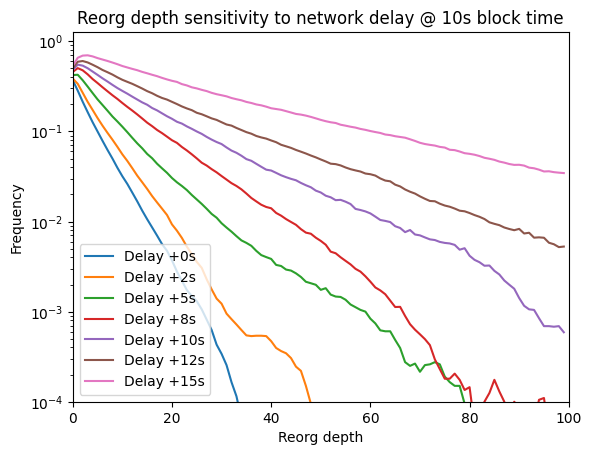
\includegraphics[width=\textwidth/2]{figs/reorg-OP-10s-no_blend-2M-OK.png}}
\subfloat[20 seconds block time, $f=0.05$]{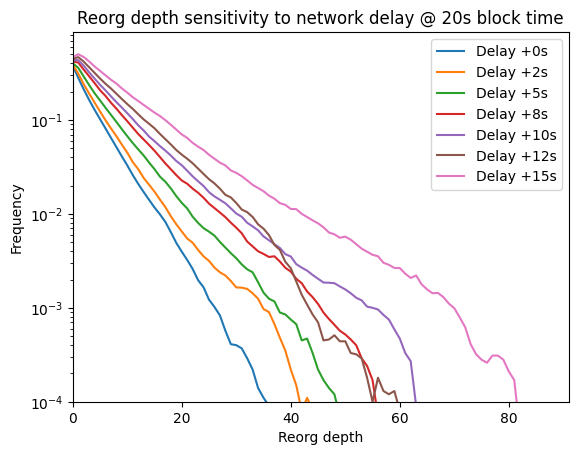
\includegraphics[width=\textwidth/2]{figs/reorg-OP-20s-no_blend-2M-OK.png}}\\
\subfloat[33 seconds block time, $f=0.03$]{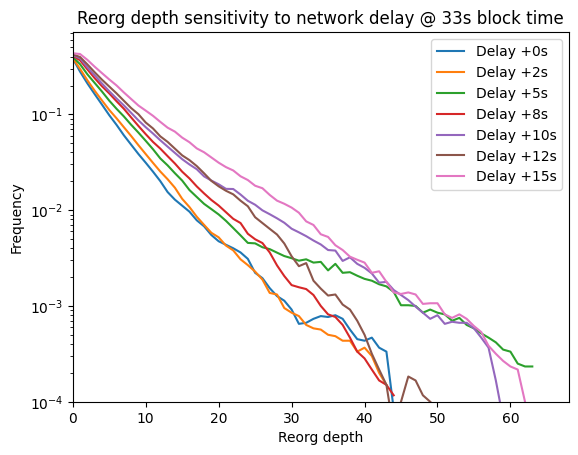
\includegraphics[width=\textwidth/2]{figs/reorg-OP-33s-no_blend-2M-OK.png}}
\subfloat[40 seconds block time, $f=0.025$]{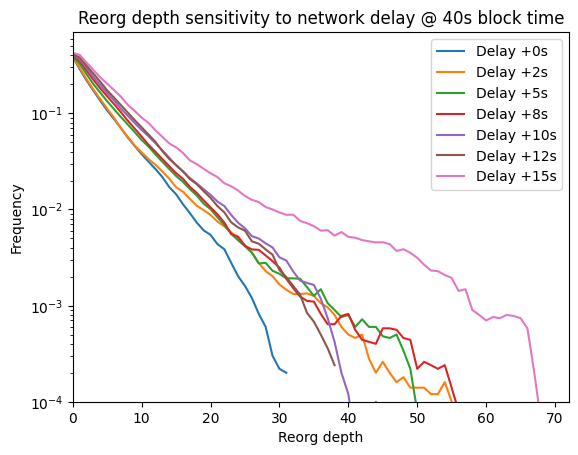
\includegraphics[width=\textwidth/2]{figs/reorg-OP-40s-no_blend-2M-OK.png}}
\caption{Impact of network delay on the reorg depth for Ouroboros Praos and \ProjBase (no parallelization, no window) with 30\% adversarial stake.}
\label{fig:delay}
\end{figure}

\begin{figure}[htbp!]
\subfloat[$f=0.05$ and $\Delta=2$s]{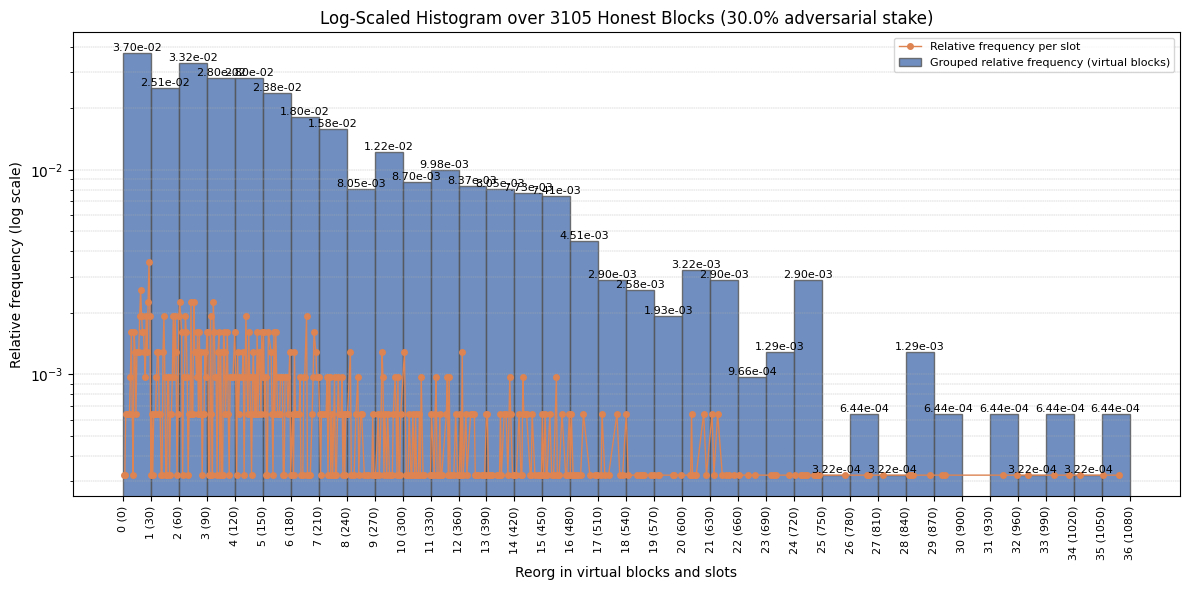
\includegraphics[width=\textwidth/3]{figs/reorg-C2-f0.05-no_blend-d2s-w30-100k-mr1069-sa0.png}}
\subfloat[$f=0.1$ and $\Delta=2$s]{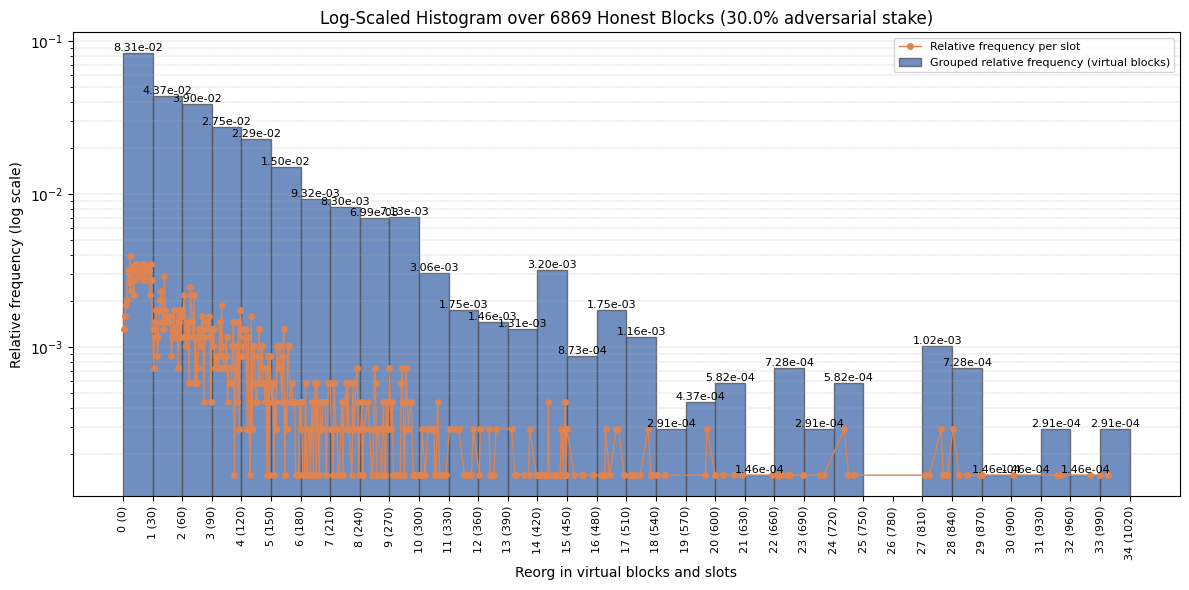
\includegraphics[width=\textwidth/3]{figs/reorg-C2-f0.1-no_blend-d2s-w30-100k-mr998-sa0}}
\subfloat[$f=0.2$ and $\Delta=2$s]{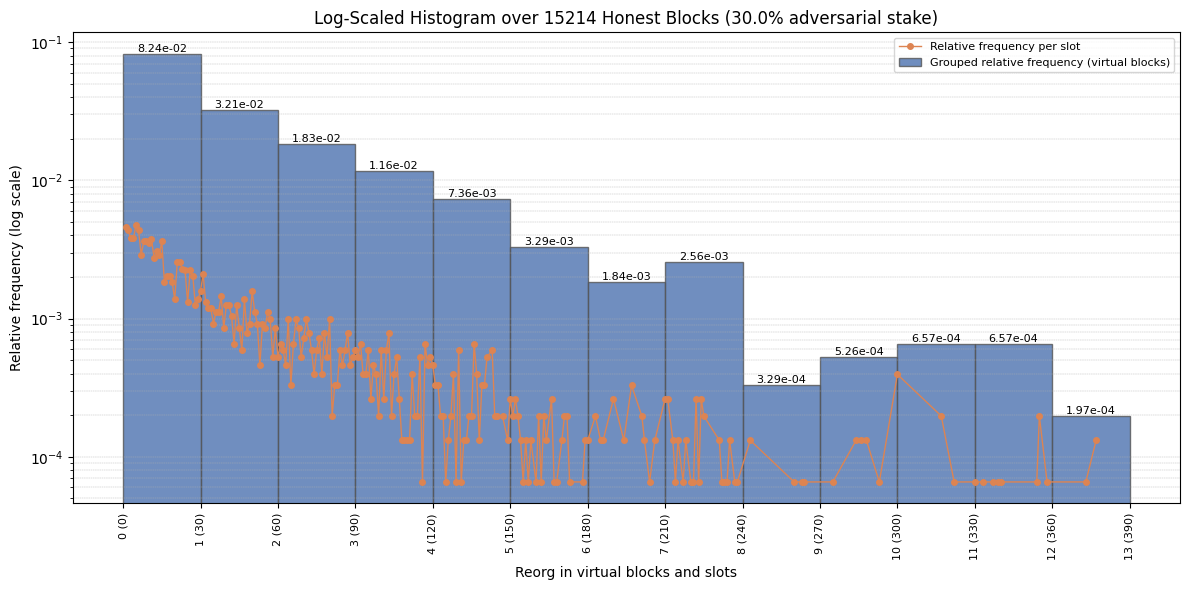
\includegraphics[width=\textwidth/3]{figs/reorg-C2-f0.2-no_blend-d2s-w30-100k-mr377-sa0}}\\
\subfloat[$f=0.05$ and $\Delta=5$s]{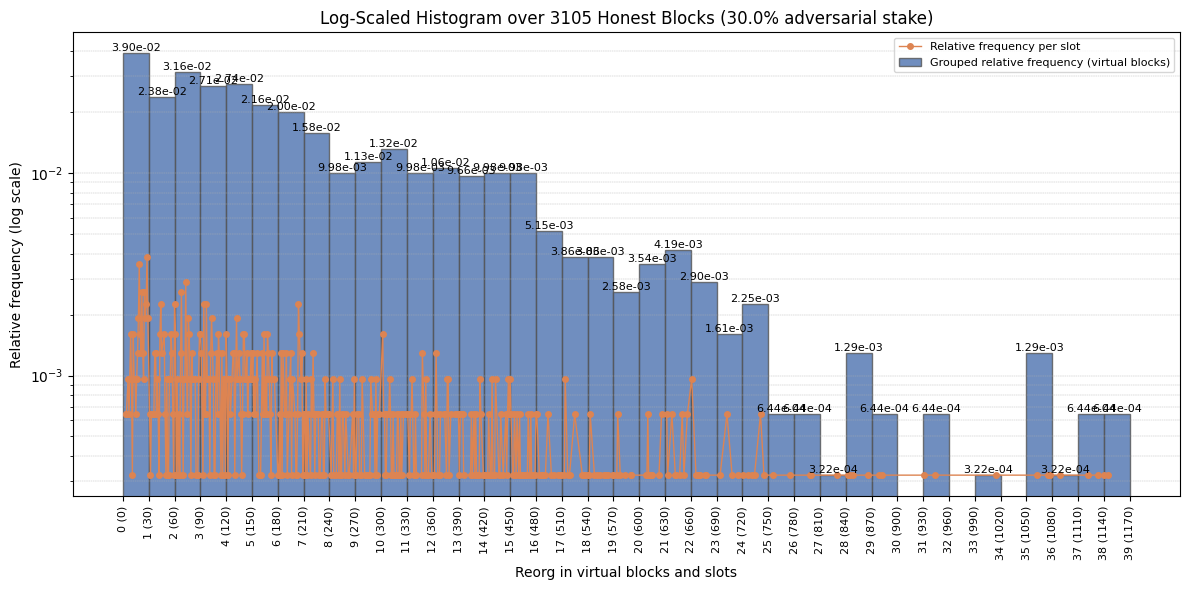
\includegraphics[width=\textwidth/3]{figs/reorg-C2-f0.05-no_blend-d5s-w30-100k-mr1145-sa0.png}}
\subfloat[$f=0.1$ and $\Delta=5$s]{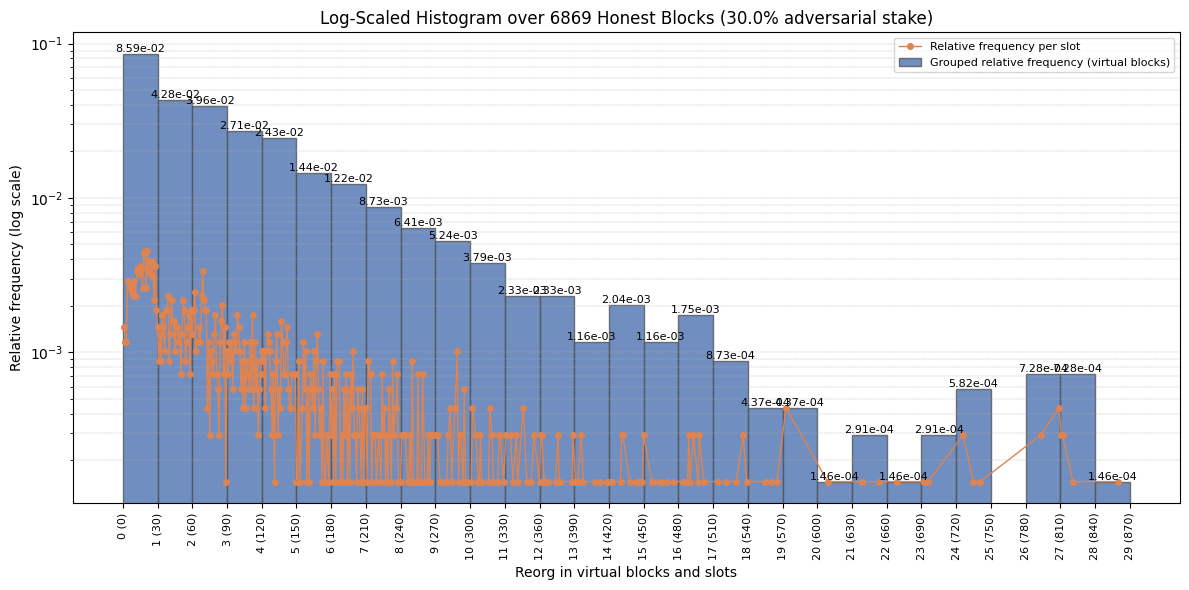
\includegraphics[width=\textwidth/3]{figs/reorg-C2-f0.1-no_blend-d5s-w30-100k-mr860-sa0}}
\subfloat[$f=0.2$ and $\Delta=5$s]{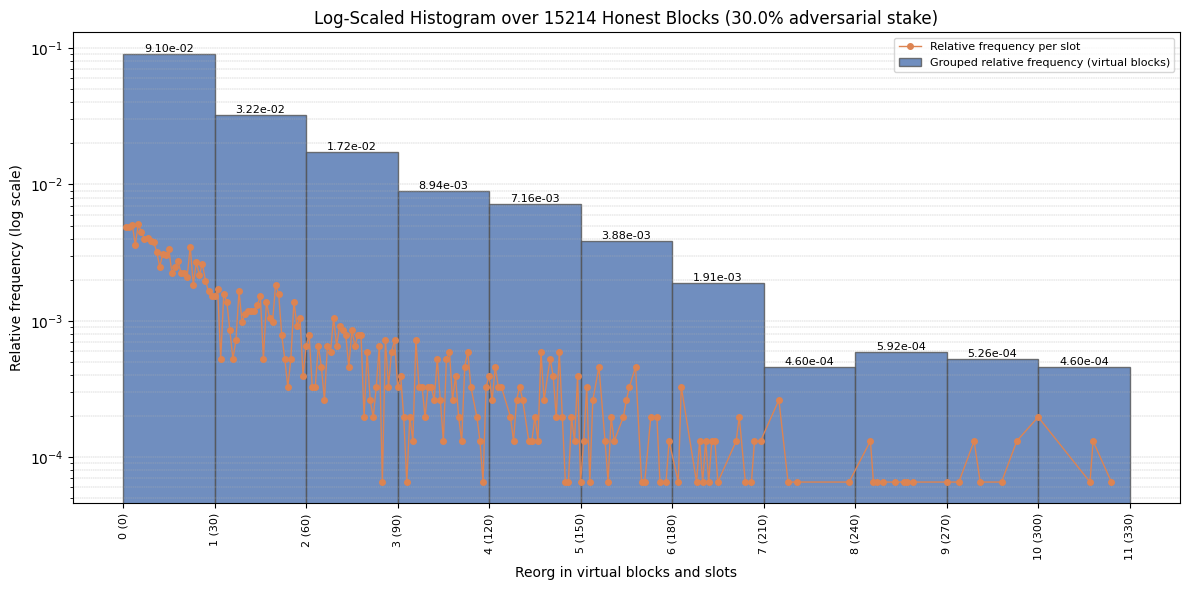
\includegraphics[width=\textwidth/3]{figs/reorg-C2-f0.2-no_blend-d5s-w30-100k-mr324-sa0}}\\
\subfloat[$f=0.05$ and $\Delta=8$s]{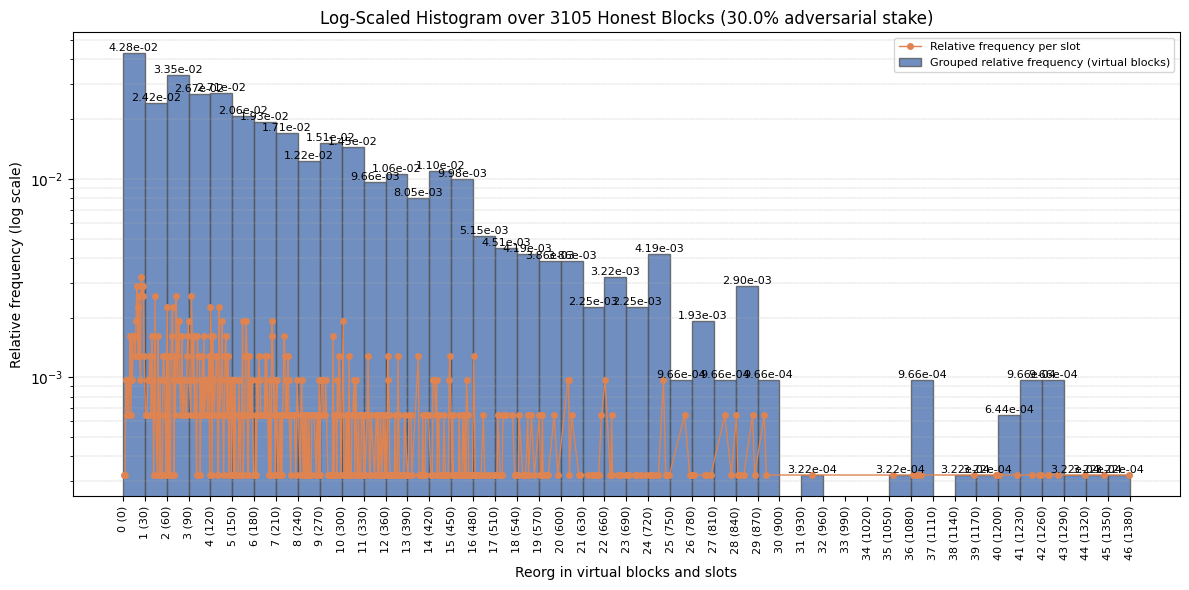
\includegraphics[width=\textwidth/3]{figs/reorg-C2-f0.05-no_blend-d8s-w30-100k-mr1379-sa0.png}}
\subfloat[$f=0.1$ and $\Delta=8$s]{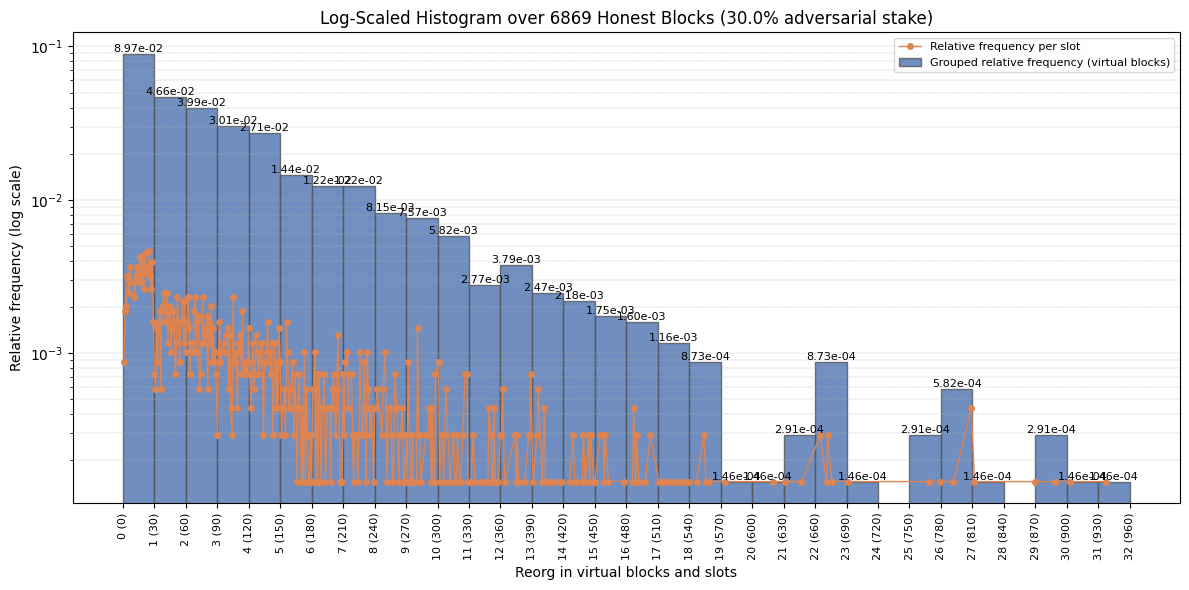
\includegraphics[width=\textwidth/3]{figs/reorg-C2-f0.1-no_blend-d8s-w30-100k-mr937-sa0}}
\subfloat[$f=0.2$ and $\Delta=8$s]{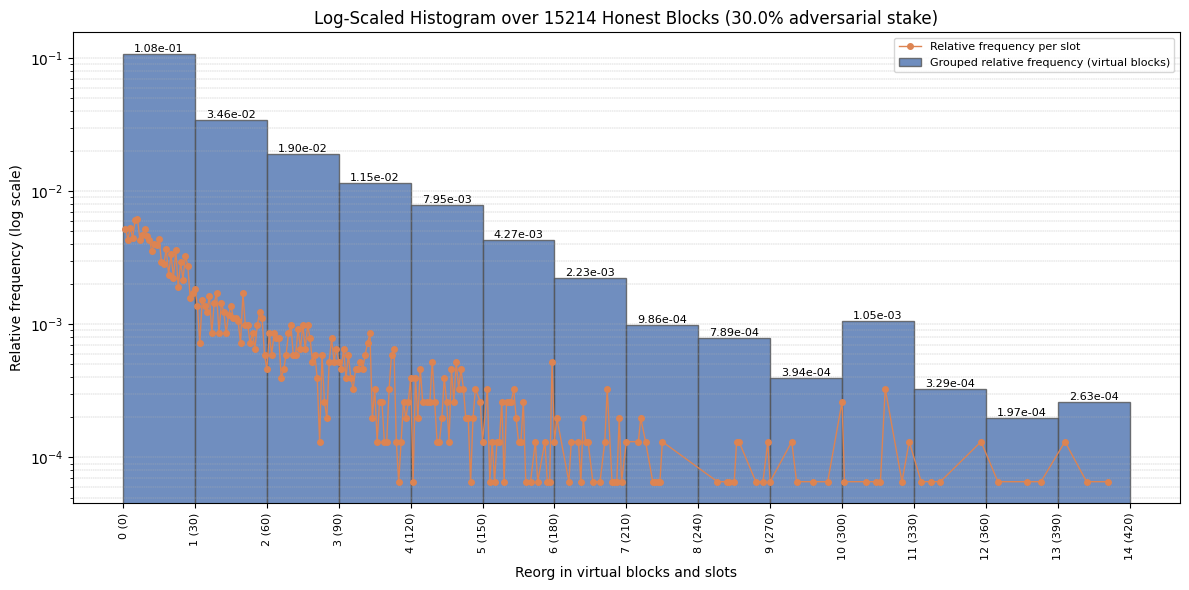
\includegraphics[width=\textwidth/3]{figs/reorg-C2-f0.2-no_blend-d8s-w30-100k-mr411-sa0}}\\
\subfloat[$f=0.05$ and $\Delta=10$s]{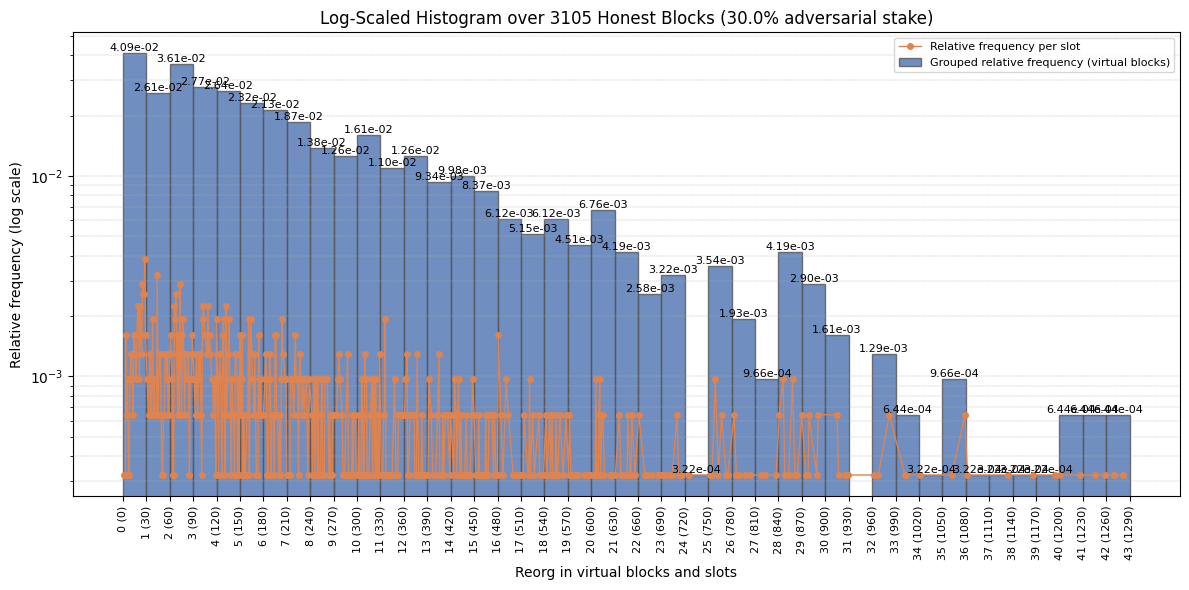
\includegraphics[width=\textwidth/3]{figs/reorg-C2-f0.05-no_blend-d10s-w30-100k-mr1282-sa0.png}}
\subfloat[$f=0.1$ and $\Delta=10$s]{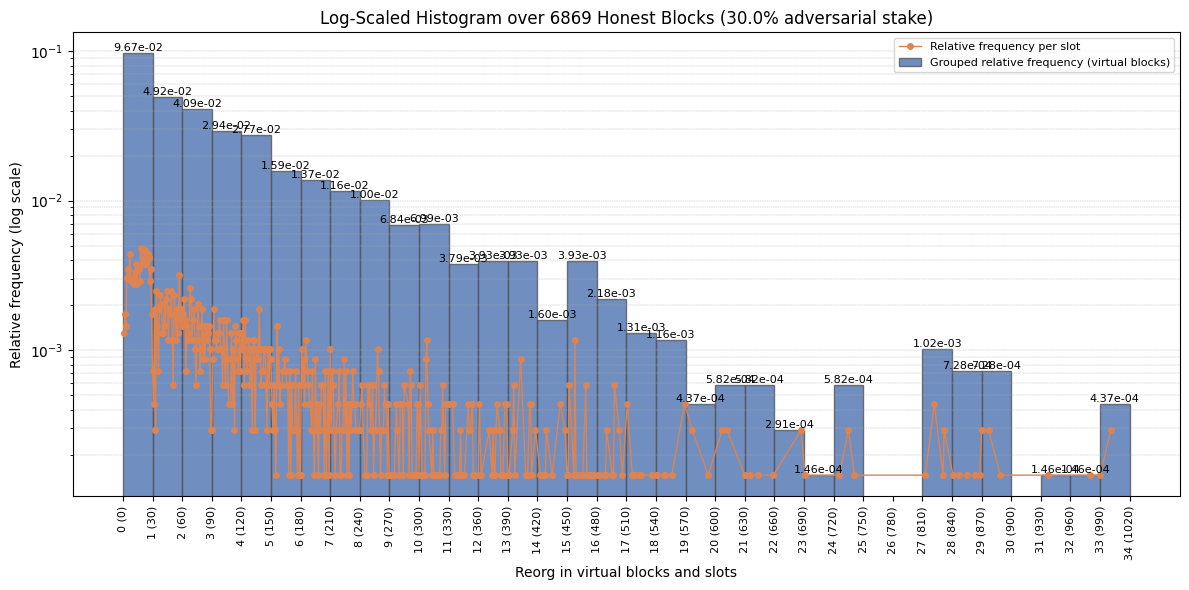
\includegraphics[width=\textwidth/3]{figs/reorg-C2-f0.1-no_blend-d10s-w30-100k-mr1001-sa0}}
\subfloat[$f=0.2$ and $\Delta=10$s]{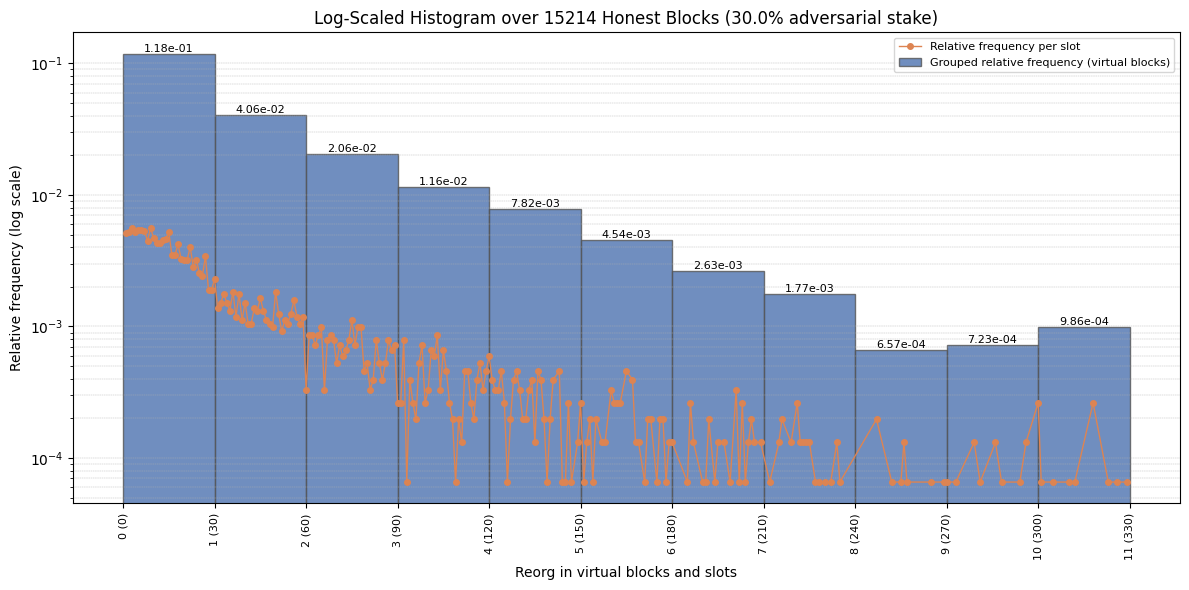
\includegraphics[width=\textwidth/3]{figs/reorg-C2-f0.2-no_blend-d10s-w30-100k-mr329-sa0}}\\
\subfloat[$f=0.05$ and $\Delta=12$s]{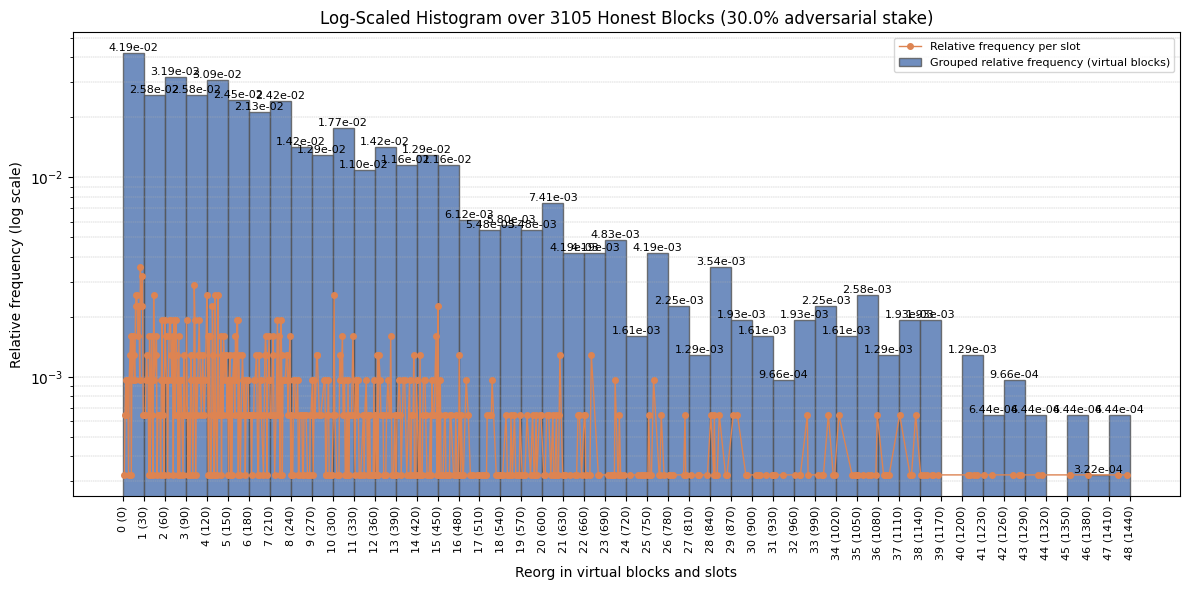
\includegraphics[width=\textwidth/3]{figs/reorg-C2-f0.05-no_blend-d12s-w30-100k-mr1436-sa0.png}}
\subfloat[$f=0.1$ and $\Delta=12$s]{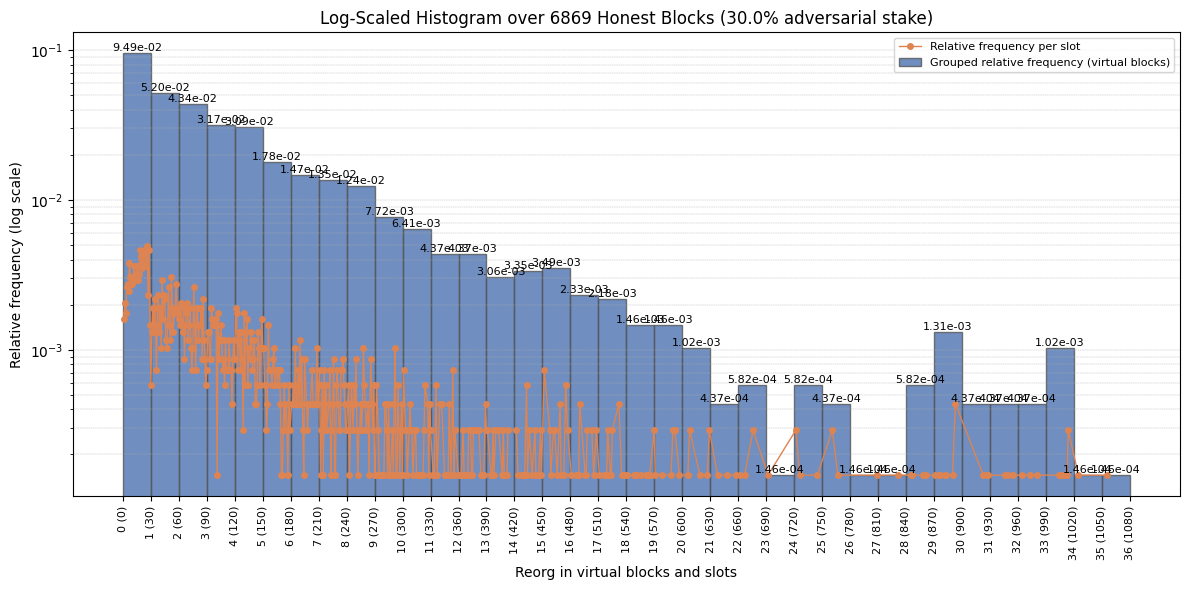
\includegraphics[width=\textwidth/3]{figs/reorg-C2-f0.1-no_blend-d12s-w30-100k-mr1056-sa0}}
\subfloat[$f=0.2$ and $\Delta=12$s]{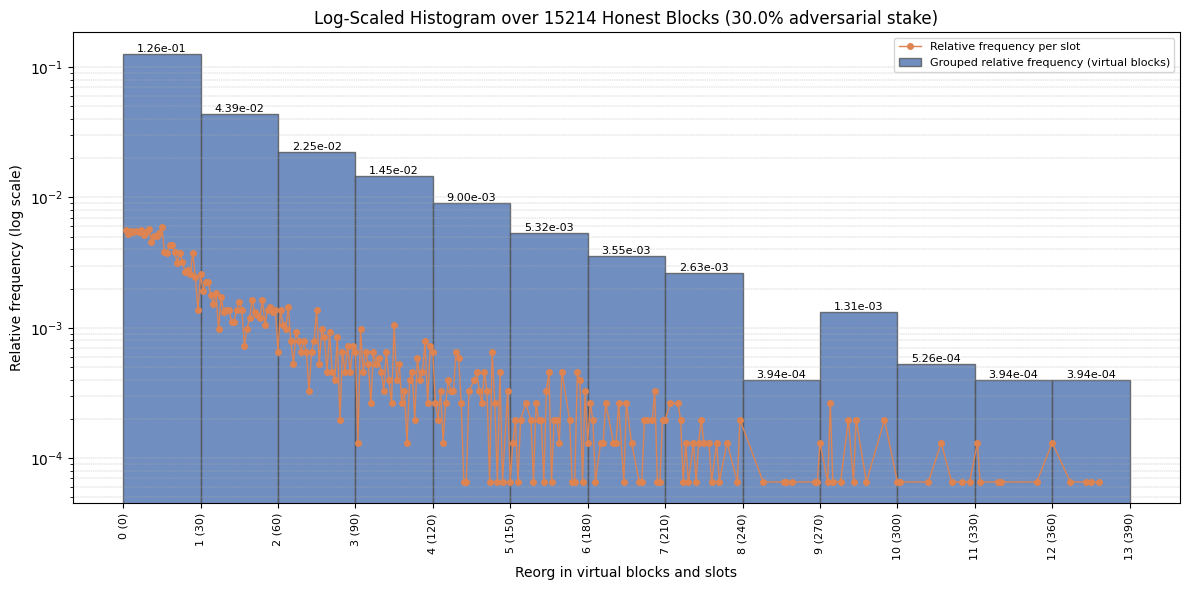
\includegraphics[width=\textwidth/3]{figs/reorg-C2-f0.2-no_blend-d12s-w30-100k-mr378-sa0}}\\
\subfloat[$f=0.05$ and $\Delta=15$s]{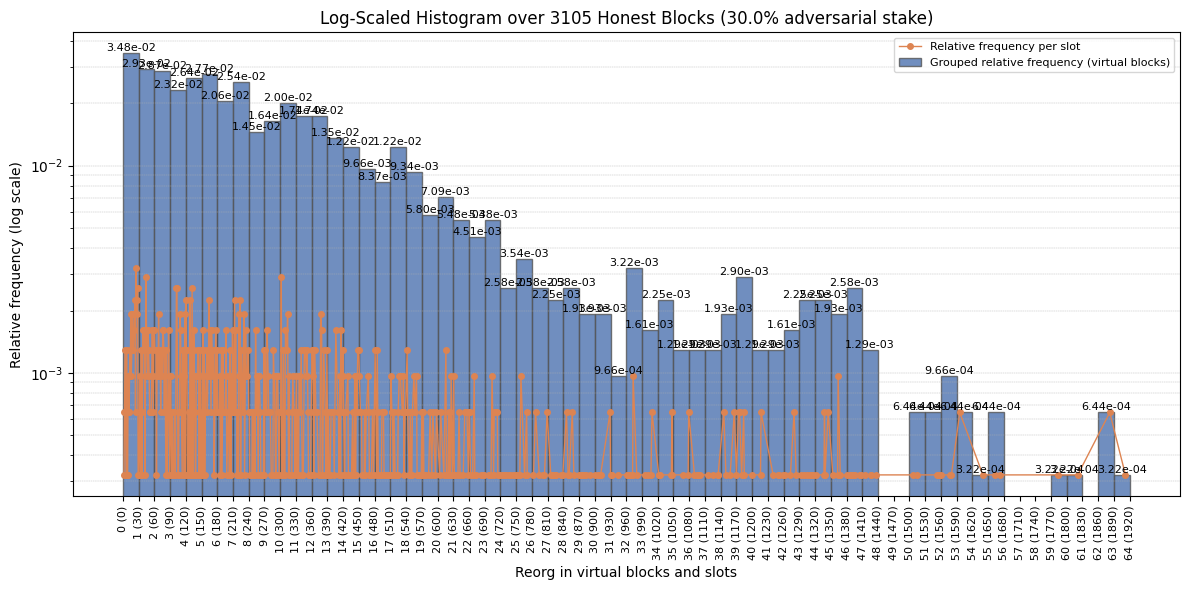
\includegraphics[width=\textwidth/3]{figs/reorg-C2-f0.05-no_blend-d15s-w30-100k-mr1912-sa0.png}}
\subfloat[$f=0.1$ and $\Delta=15$s]{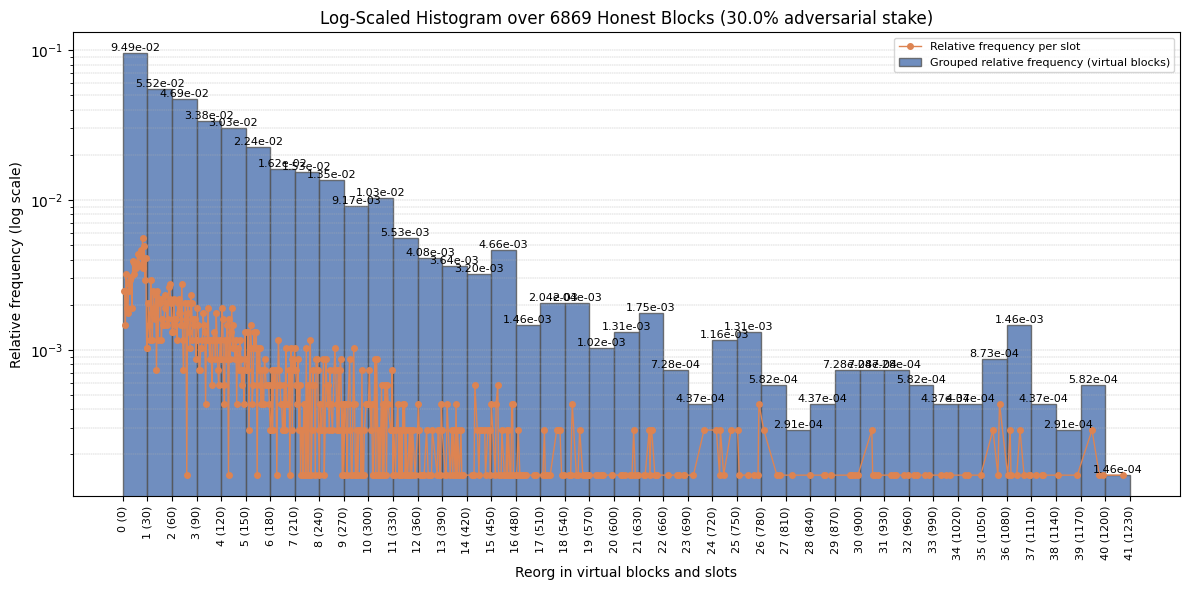
\includegraphics[width=\textwidth/3]{figs/reorg-C2-f0.1-no_blend-d15s-w30-100k-mr1222-sa0}}
\subfloat[$f=0.2$ and $\Delta=15$s]{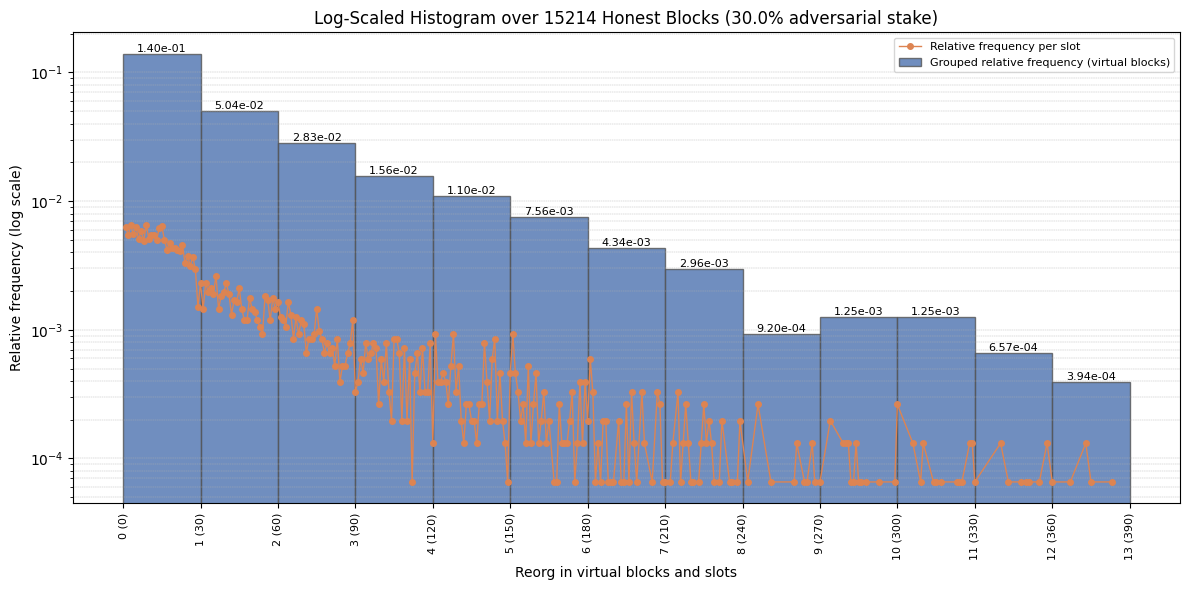
\includegraphics[width=\textwidth/3]{figs/reorg-C2-f0.2-no_blend-d15s-w30-100k-mr383-sa0}}\\
\caption{Impact of block production rate and mean broadcast delay on the reorg depth for \ProjBase with 30s window and 30\% adversarial stake.\mnote{This could be moved to appendix as I'm extracting info from here in the Fig.~\ref{fig:delay-plot}.}}
\label{fig:c2-delay}
\end{figure}

\begin{figure}[htbp!]
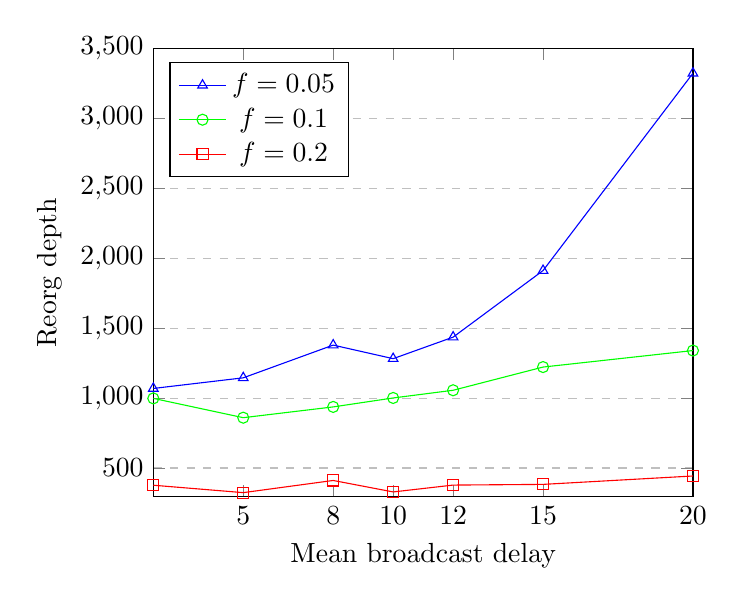
\begin{tikzpicture}
\begin{axis}[
    %title={Impact of window size on the reorg depth of \ProjBase with 30\% adversarial stake and $f=0.25$},
    xlabel={Mean broadcast delay},
    ylabel={Reorg depth},
    xmin=2, xmax=20,
    ymin=294, ymax=3500,
    xtick={1,5,8,10,12,15,20},
    ytick={500,1000,1500,2000,2500,3000,3500},
    legend pos=north west,
    ymajorgrids=true,
    grid style=dashed,
]

\addplot[
    color=blue,
    mark=triangle,
    ]
    coordinates {
    (2,1069)(5,1145)(8,1379)(10,1282)(12,1436)(15,1912)(20,3323)(30,5000)
    };
    \addlegendentry{$f=0.05$}
\addplot[
    color=green,
    mark=o,
    ]
    coordinates {
    (2,998)(5,860)(8,937)(10,1001)(12,1056)(15,1222)(20,1340)(30,2000)
    };
    \addlegendentry{$f=0.1$}
\addplot[
    color=red,
    mark=square,
    ]
    coordinates {
    (2,377)(5,324)(8,411)(10,329)(12,378)(15,383)(20,443)(30,1000)
    };
    \addlegendentry{$f=0.2$}
    
\end{axis}
\end{tikzpicture}
\caption{Relation between mean block production rate and broadcast delay on the reorg depth of \ProjBase with 30\% adversarial stake, and window size of 30 slots. When the mean broadcast delay increases, the reorg depth also increases. However, when the block production rate increases, the amplitude of reorg depth increase becomes smaller. In other words, with higher block production, the reorg depth becomes less sensitive to the delay.}
\label{fig:delay-plot}
\end{figure}


%\begin{figure}[htbp!]
%\subfloat[10 slots window length]{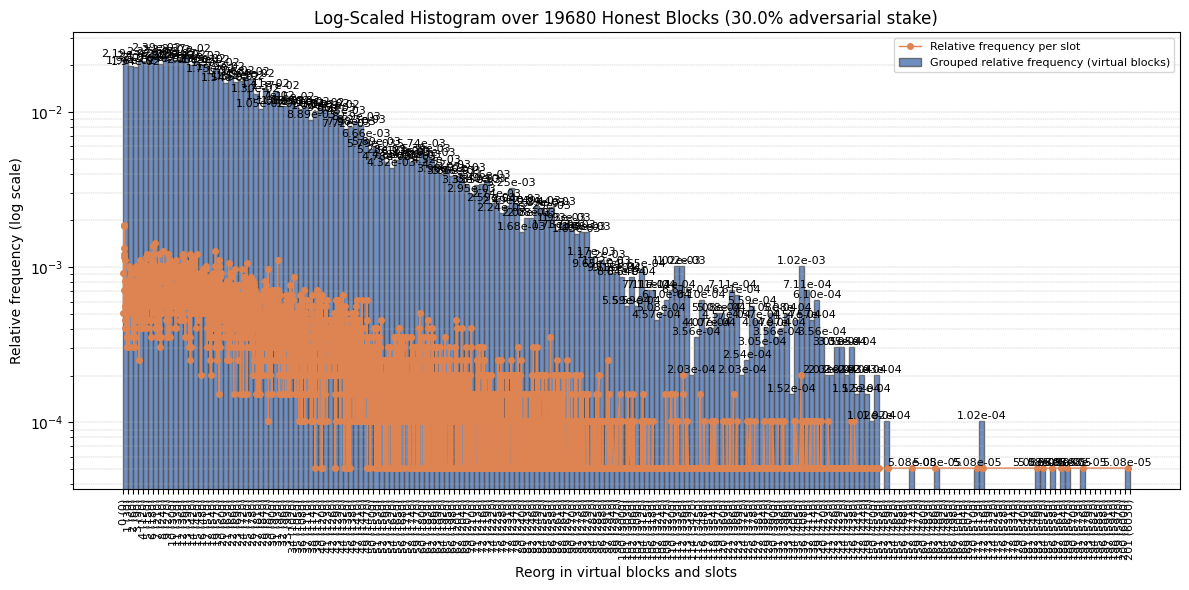
\includegraphics[width=\textwidth]{figs/reorg-C2-f0.25-no_blend-d20s-w10-100k.png}}\\
%\subfloat[20 slots window length]{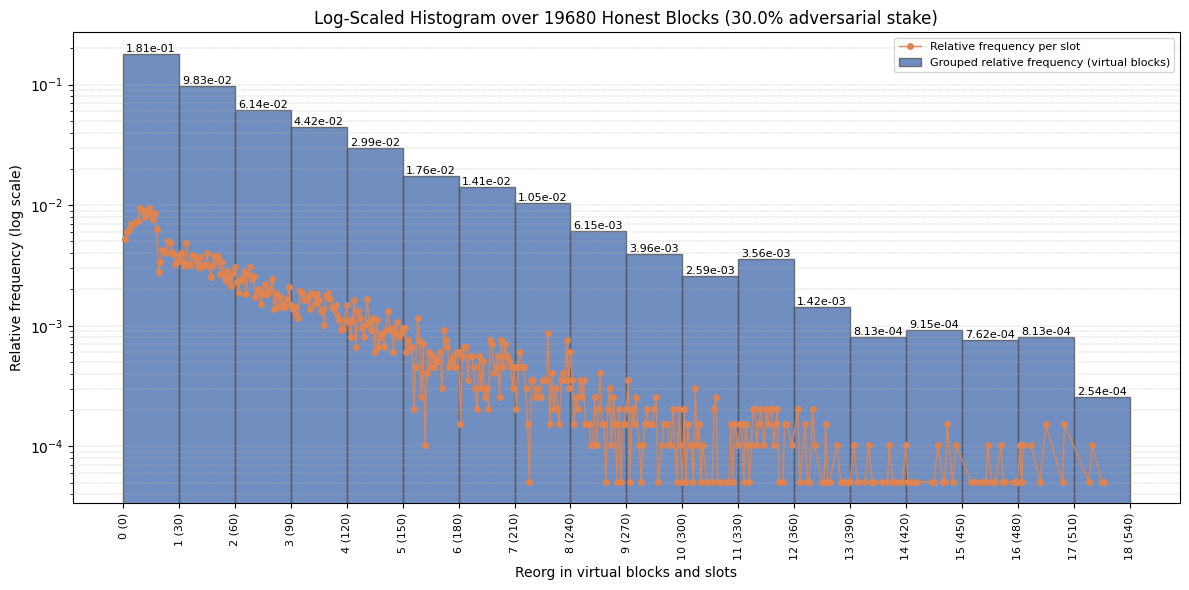
\includegraphics[width=\textwidth/2]{figs/reorg-C2-f0.25-no_blend-d20s-w20-100k.png}}
%\subfloat[30 slots window length]{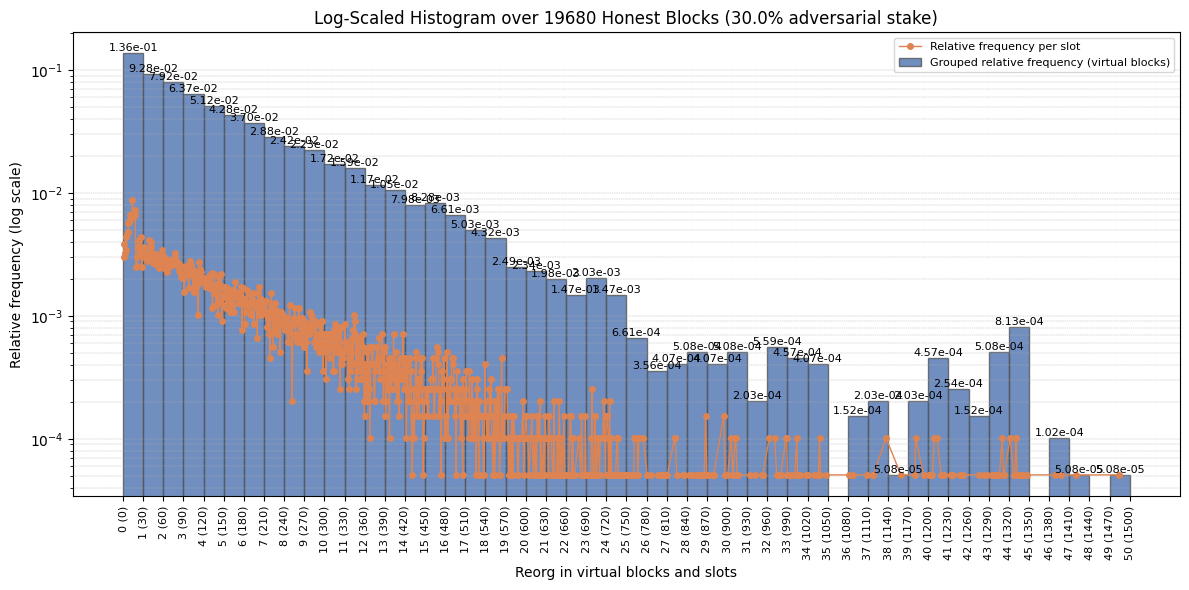
\includegraphics[width=\textwidth/2]{figs/reorg-C2-f0.25-no_blend-d20s-w30-100k.png}}
%\caption{Impact of window size on the reorg depth of \ProjBase with 30\% adversarial stake and $f=0.25$.}
%\label{fig:window}
%\end{figure}

\begin{figure}[htbp!]
\subfloat[15 seconds mean broadcast delay]{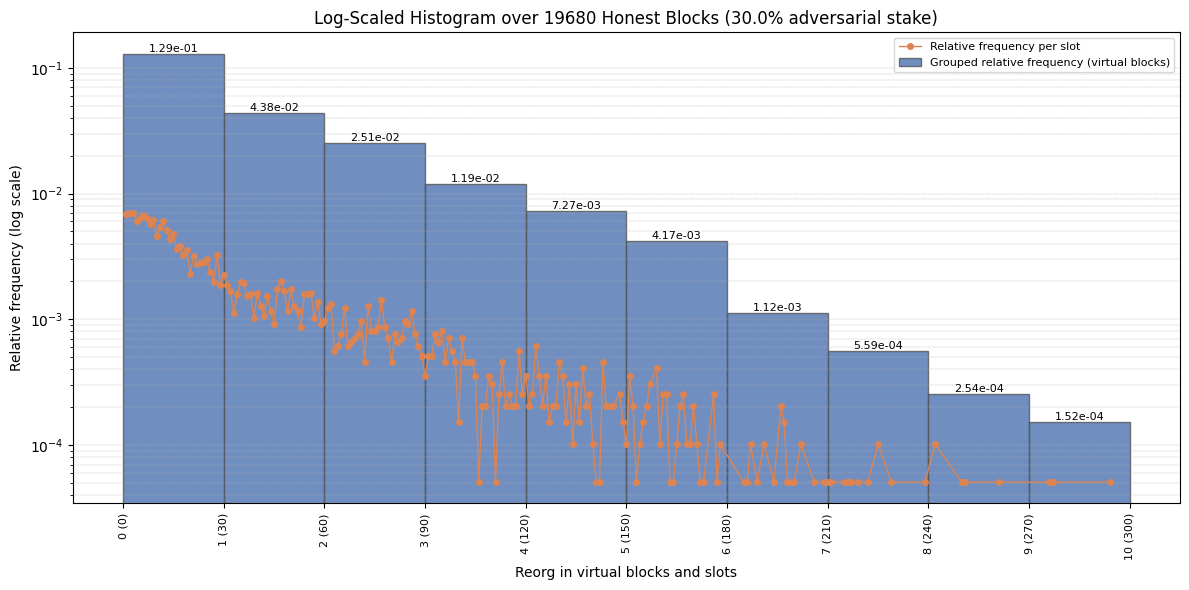
\includegraphics[width=\textwidth/3]{figs/reorg-C2-f0.25-no_blend-d15s-w30-100k-mr294-sa0.png}}
\subfloat[25 seconds mean broadcast delay]{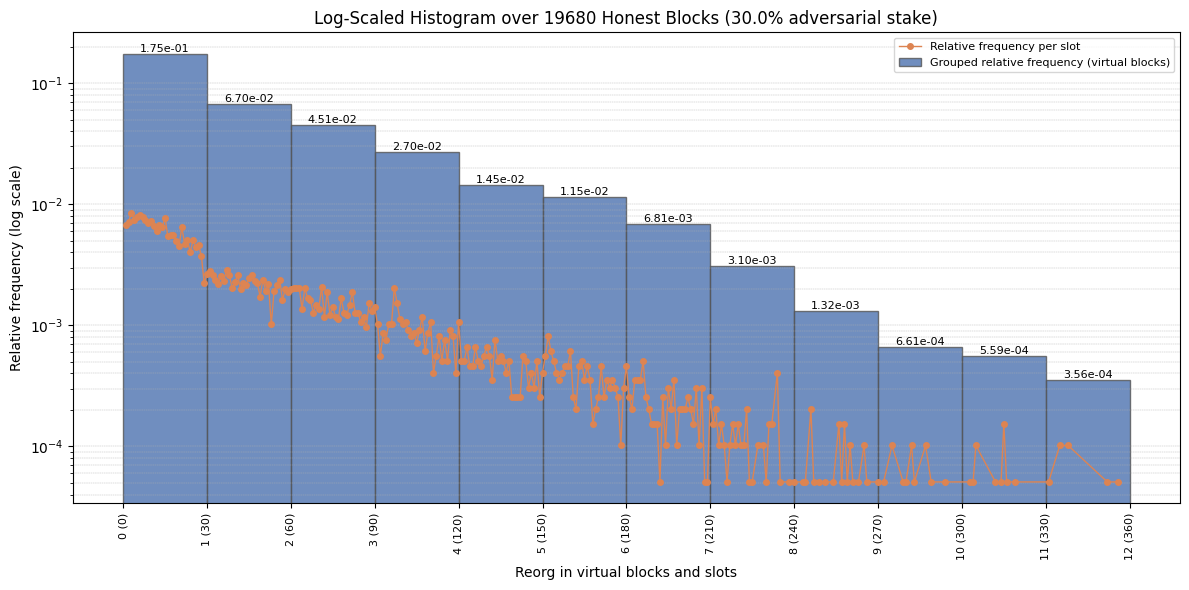
\includegraphics[width=\textwidth/3]{figs/reorg-C2-f0.25-no_blend-d25s-w30-100k-mr356-sa0.png}}
\subfloat[30 seconds mean broadcast delay]{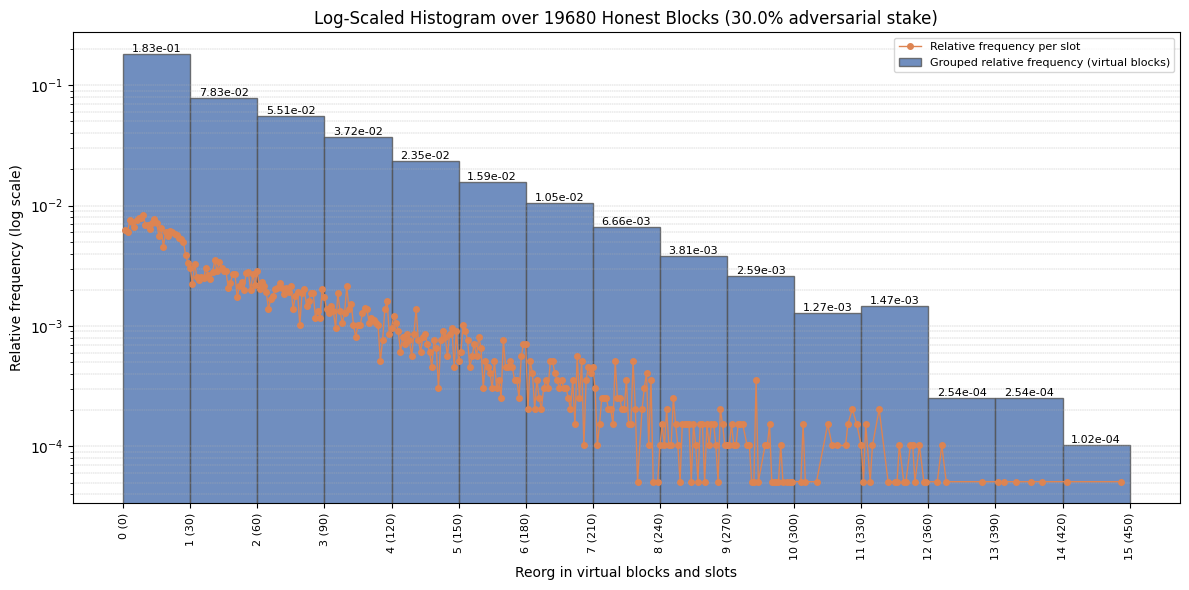
\includegraphics[width=\textwidth/3]{figs/reorg-C2-f0.25-no_blend-d30s-w30-100k-mr446-sa0.png}}\\
\subfloat[35 seconds mean broadcast delay]{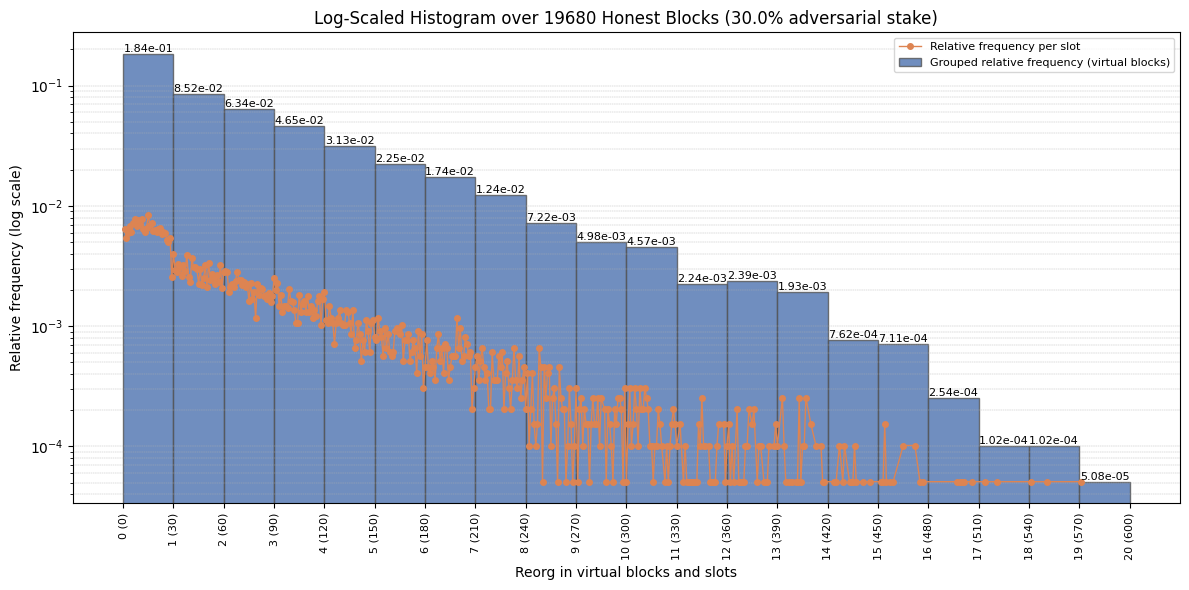
\includegraphics[width=\textwidth/3]{figs/reorg-C2-f0.25-no_blend-d35s-w30-100k-mr571-sa0.png}}
\subfloat[40 seconds mean broadcast delay]{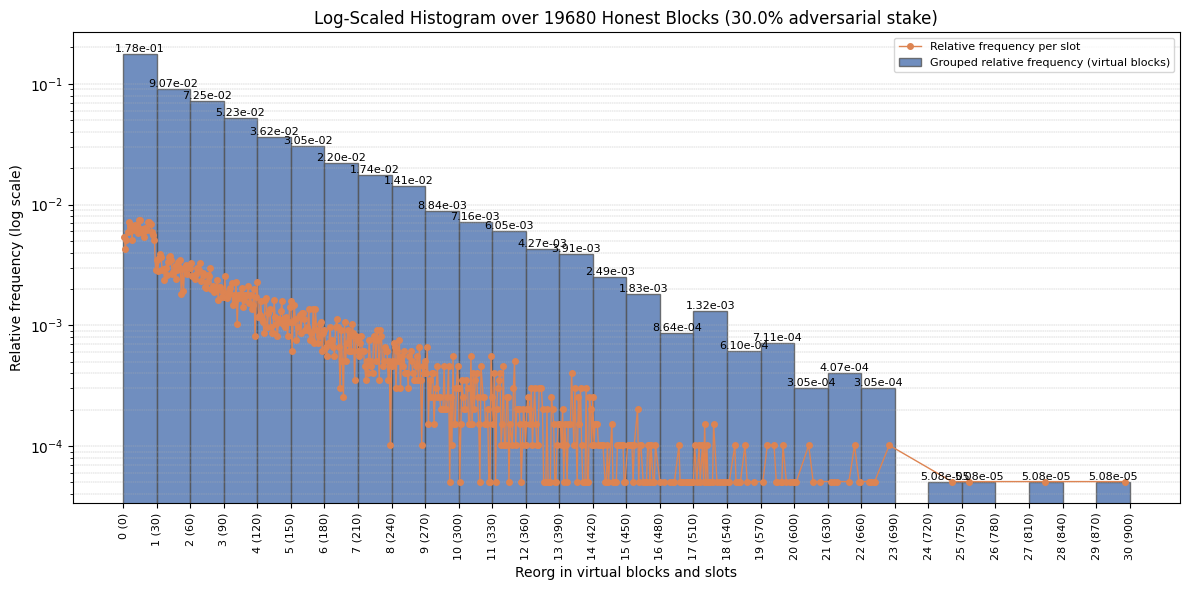
\includegraphics[width=\textwidth/3]{figs/reorg-C2-f0.25-no_blend-d40s-w30-100k-mr896-sa0.png}}
\subfloat[50 seconds mean broadcast delay]{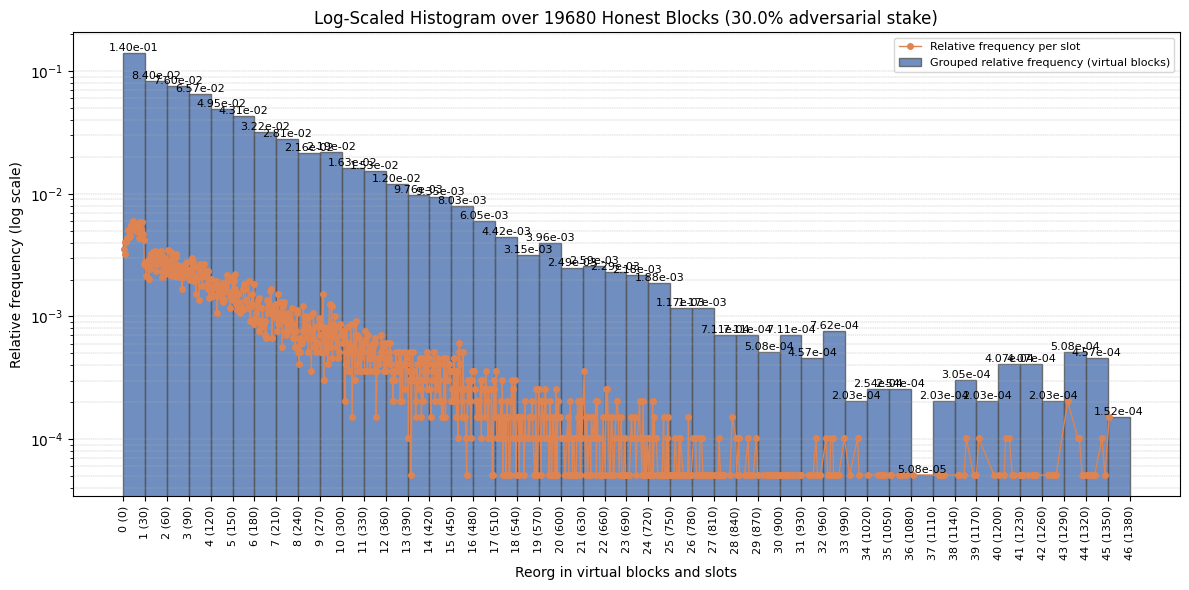
\includegraphics[width=\textwidth/3]{figs/reorg-C2-f0.25-no_blend-d50s-w30-100k-mr1352-sa0.png}}\\
\subfloat[55 seconds mean broadcast delay]{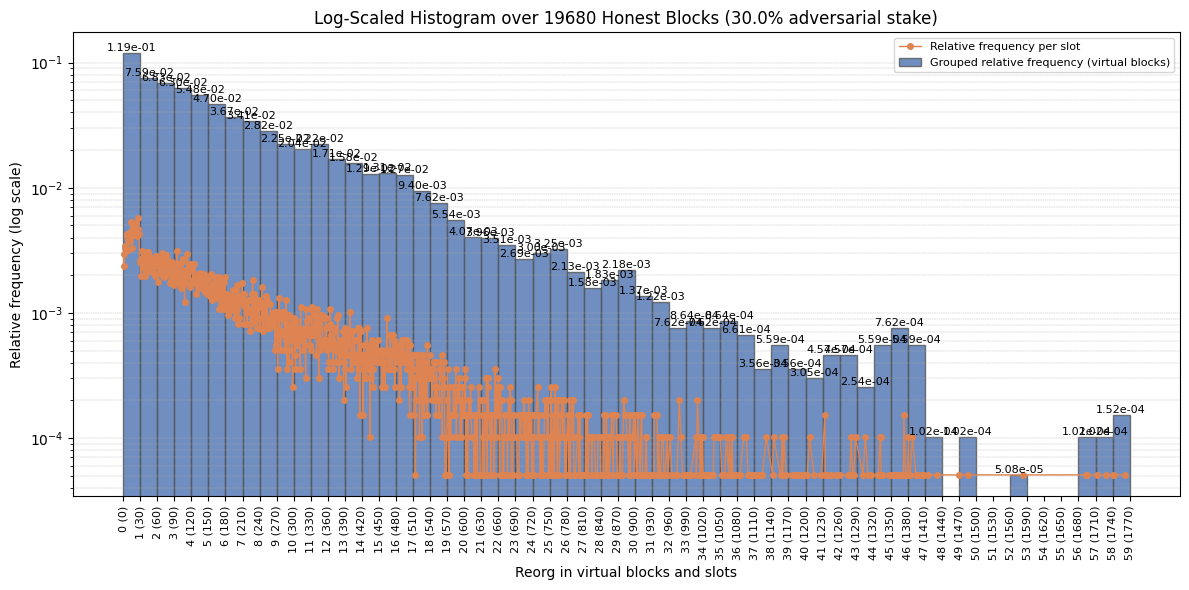
\includegraphics[width=\textwidth/3]{figs/reorg-C2-f0.25-no_blend-d55s-w30-100k-mr1762-sa0.png}}
\subfloat[60 seconds mean broadcast delay]{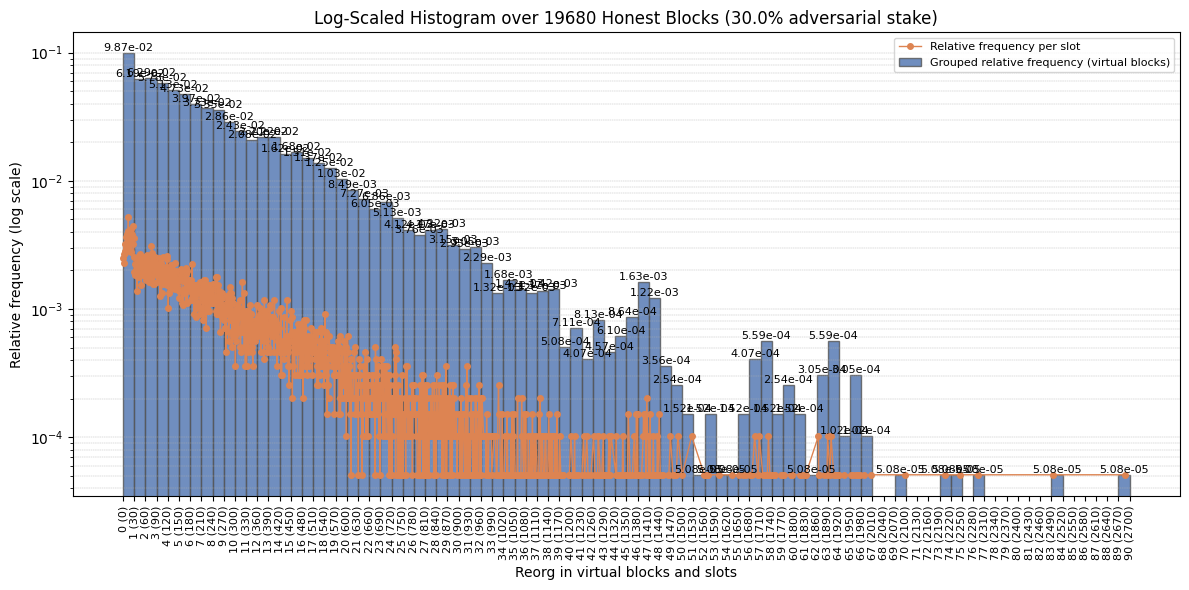
\includegraphics[width=\textwidth/3]{figs/reorg-C2-f0.25-no_blend-d60s-w30-100k-mr2687-sa3.png}}
\subfloat[65 seconds mean broadcast delay]{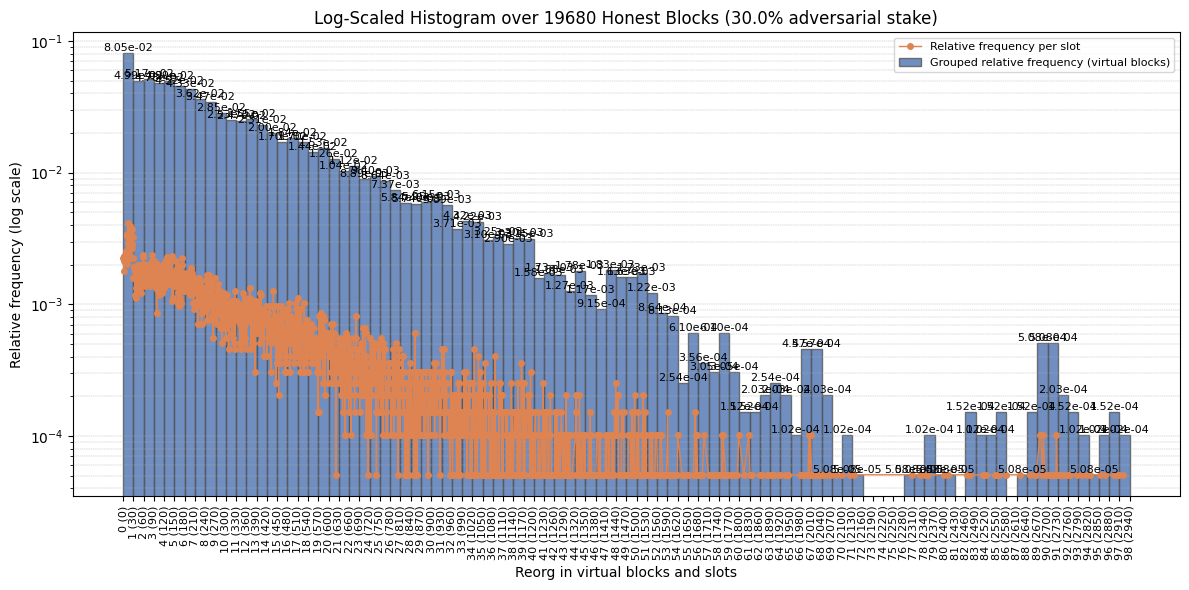
\includegraphics[width=\textwidth/3]{figs/reorg-C2-f0.25-no_blend-d65s-w30-100k-mr2920-sa51.png}}\\
\subfloat[70 seconds mean broadcast delay]{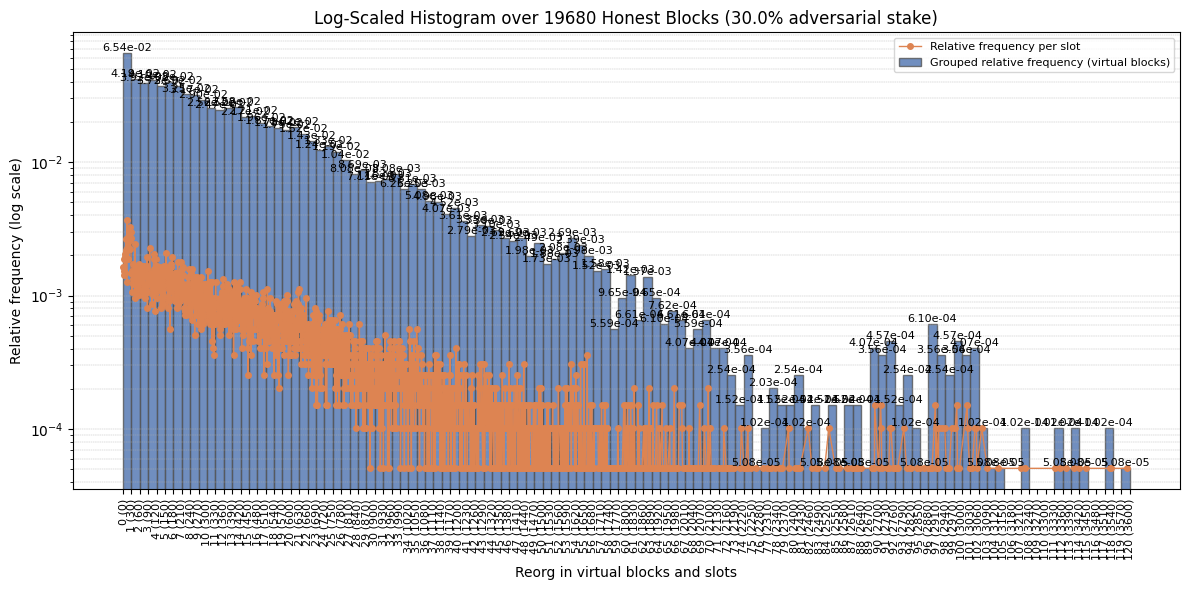
\includegraphics[width=\textwidth/3]{figs/reorg-C2-f0.25-no_blend-d70s-w30-100k-mr3591-sa92.png}}
\subfloat[80 seconds mean broadcast delay]{\includegraphics[width=\textwidth/3]{figs/reorg-C2-f0.25-no_blend-d80s-w30-100k-mr5156-sa282.png}}
\subfloat[90 seconds mean broadcast delay]{\includegraphics[width=\textwidth/3]{figs/reorg-C2-f0.25-no_blend-d90s-w30-100k-mr7658-sa700.png}}\\
\caption{Impact of the mean broadcast delay on the reorg depth of \ProjBase with 30\% adversarial stake, window size 30 slots, and $f=0.25$. The reorg depth increases as the mean broadcast delay increases.\mnote{We might move this to the appendix as the Fig.~\ref{fig:window-attack} extracts information from it.}}
\label{fig:window}
\end{figure}

\begin{figure}[htbp!]
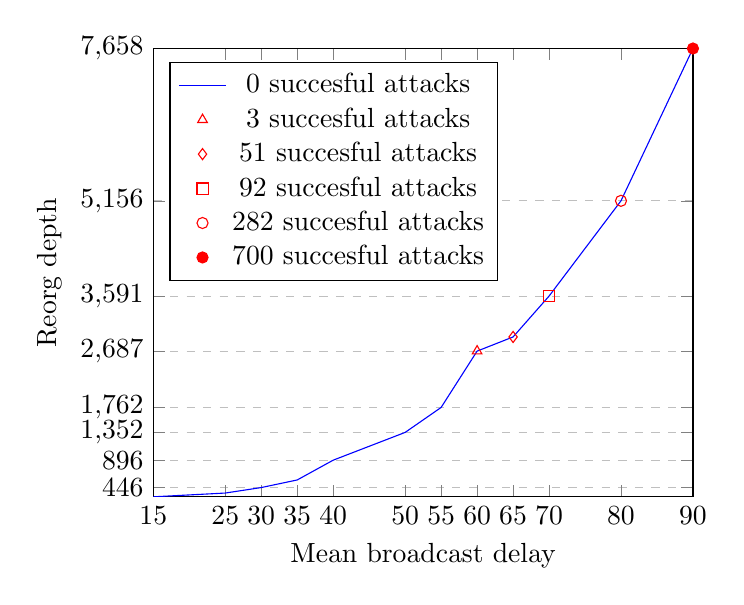
\begin{tikzpicture}
\begin{axis}[
    %title={Impact of window size on the reorg depth of \ProjBase with 30\% adversarial stake and $f=0.25$},
    xlabel={Mean broadcast delay},
    ylabel={Reorg depth},
    xmin=15, xmax=90,
    ymin=294, ymax=7658,
    xtick={15,25,30,35,40,50,55,60,65,70,80,90},
    ytick={446,896,1352,1762,2687,3591,5156,7658},
    legend pos=north west,
    ymajorgrids=true,
    grid style=dashed,
]

\addplot[
    color=blue,
    ]
    coordinates {
    (15,294)(25,356)(30,446)(35,571)(40,896)(50,1352)(55,1762)(60,2687)(65,2920)(70,3591)(80,5156)(90,7658)
    };
    \addlegendentry{0 succesful attacks}
\addplot[
    only marks,
    color=red,
    mark=triangle,
    ]
    coordinates {
    (60,2687)
    };
    \addlegendentry{3 succesful attacks}
\addplot[
    only marks,
    color=red,
    mark=diamond,
    ]
    coordinates {
    (65,2920)
    };
    \addlegendentry{51 succesful attacks} %0.26%
\addplot[
    only marks,
    color=red,
    mark=square,
    ]
    coordinates {
    (70,3591)
    };
    \addlegendentry{92 succesful attacks}
\addplot[
    only marks,
    color=red,
    mark=o,
    ]
    coordinates {
    (80,5156)
    };
    \addlegendentry{282 succesful attacks} %1.43%
\addplot[
    only marks,
    color=red,
    mark=*,
    ]
    coordinates {
    (90,7658)
    };
    \addlegendentry{700 succesful attacks} %3.56%
    
\end{axis}
\end{tikzpicture}
\caption{Relation between mean broadcast delay on the reorg depth of \ProjBase with 30\% adversarial stake, window size of 30 slots and $f=0.25$. When the mean broadcast delay exceeds the window size, the reorg depth commences to increase exponentially. Successful attacks become probable when the mean broadcast delay approaches double the window size. Consequently, $w \geq \Delta$ ensures that the reorg depth remains low, thereby reducing the likelihood of executing a successful attack. Conversely, $2\Delta < w < \Delta$ results in a higher reorg depth, while $w \leq 2\Delta$ significantly increases the probability of successful attacks.}
\label{fig:window-attack}
\end{figure}

\paragraph{Network delay.}
Holding $\alpha=0.3$, increasing $\Delta$ relative to slot time induces more transient forks (Fig.~\ref{fig:delay} and Fig.~\ref{fig:c2-delay}) but, if $w\ge\Delta$, they resolve within $w$ slots and the reorg-depth distribution shifts only slightly. If $w<\Delta$, reorgs can grow unbounded (e.g., $w=30$ and $\Delta=60$ slots Fig.~\ref{fig:window}g), with tips oscillating indefinitely and successful attacks emerging (Fig.~\ref{fig:window-attack}). This confirms the necessity of $w\ge\Delta$ for security, matching the TB requirement.

%ADVERSARY_STAKE = 0.30
%# Run multiple experiments
%attacked_results, total_blocks, sim = run_multiple_attacks(
%    n_runs=1,
%    slots=100000,
%    f=0.25,
%    window_size=10,
%    use_deps=True,
%    adversary_control=ADVERSARY_STAKE,
%    #network=no_blend_net,
%    network=replace(no_blend_net, broadcast_delay_mean=20), # i in [0,2,5,8,10,12,15]
%    base_seed=0,
%    # these are honest blocks that won't be attacked and will not count in the stats, but give room for the attack.
%    skip_last=500
%)
%Largest reorg length: 6018 (~200 virtual blocks of 30-seconds)
%Successful attacks: 53 (0.27%)
%Successful attacks list [target block, target slot, reorg length]): [[19338, 95530, 4379], [19347, 95599, 4180], [19385, 95773, 4120], [19393, 95832, 4143], [19394, 95835, 4092], [19398, 95850, 4069], [19405, 95886, 3983], [19408, 95903, 3891], [19415, 95935, 3926], [19422, 95974, 3969], [19424, 95977, 3984], [19426, 95996, 3957], [19433, 96014, 3806], [19434, 96015, 3948], [19435, 96034, 3957], [19439, 96041, 3948], [19441, 96050, 3779], [19469, 96219, 3532], [19480, 96248, 3595], [19488, 96279, 3688], [19489, 96286, 3573], [19508, 96383, 3340], [19510, 96401, 3346], [19566, 96769, 3143], [19588, 96855, 3018], [19595, 96879, 3048], [19607, 96919, 2911], [19615, 96950, 2939], [19618, 96970, 3018], [19621, 96979, 2934], [19629, 97035, 2906], [19635, 97059, 2904], [19638, 97064, 2889], [19639, 97068, 2852], [19641, 97089, 2881], [19643, 97093, 2796], [19644, 97093, 2877], [19646, 97114, 2778], [19649, 97118, 2776], [19657, 97198, 2739], [19658, 97206, 2740], [19663, 97231, 2746], [19666, 97243, 2746], [19667, 97252, 2738], [19668, 97255, 2638], [19669, 97260, 2682], [19670, 97264, 2701], [19671, 97267, 2699], [19672, 97275, 2659], [19673, 97285, 2687], [19676, 97291, 2629], [19677, 97296, 2641], [19679, 97310, 2679]]
%CPU times: user 16min 57s, sys: 2min 47s, total: 19min 45s
%Wall time: 58min 10s

%ADVERSARY_STAKE = 0.30
%# Run multiple experiments
%attacked_results, total_blocks, sim = run_multiple_attacks(
%    n_runs=1,
%    slots=100000,
%    f=0.25,
%    window_size=5,
%    use_deps=True,
%    adversary_control=ADVERSARY_STAKE,
%    #network=no_blend_net,
%    network=replace(no_blend_net, broadcast_delay_mean=10), # i in [0,2,5,8,10,12,15]
%    base_seed=0,
%    # these are honest blocks that won't be attacked and will not count in the stats, but give room for the attack.
%    skip_last=500
%)
%Largest reorg length: 17471 (~582 virtual blocks of 30-seconds)
%Successful attacks: 146 (0.74%)
%Successful attacks list [target block, target slot, reorg length]): [[18875, 93071, 6867], [18888, 93131, 6818], [18894, 93180, 6780], [18900, 93218, 6710], [18903, 93238, 6531], [18913, 93288, 6621], [18928, 93339, 6581], [18936, 93373, 6621], [18937, 93377, 6451], [18938, 93390, 6539], [18939, 93393, 6521], [18946, 93449, 6501], [18948, 93459, 6491], [18949, 93469, 6484], [18951, 93486, 6340], [18952, 93488, 6479], [18954, 93507, 6436], [18958, 93519, 6434], [18961, 93547, 6375], [18963, 93562, 6379], [18964, 93564, 6256], [18971, 93619, 6372], [18972, 93623, 6278], [18980, 93658, 6280], [18991, 93715, 6259], [18992, 93719, 6135], [19023, 93860, 5980], [19031, 93926, 6050], [19032, 93928, 5947], [19038, 93948, 5844], [19050, 93994, 5940], [19056, 94030, 5902], [19062, 94065, 5907], [19075, 94090, 5835], [19086, 94154, 5651], [19088, 94160, 5689], [19102, 94289, 5558], [19110, 94347, 5577], [19125, 94421, 5415], [19154, 94583, 5405], [19157, 94593, 5399], [19158, 94599, 4960], [19166, 94624, 5241], [19184, 94757, 5005], [19226, 94965, 4990], [19232, 94993, 4800], [19237, 95008, 4799], [19242, 95038, 4852], [19249, 95082, 4790], [19261, 95145, 4699], [19262, 95146, 4793], [19263, 95153, 4832], [19266, 95164, 4803], [19267, 95166, 4800], [19270, 95195, 4799], [19271, 95198, 4788], [19272, 95198, 4799], [19274, 95199, 4748], [19275, 95205, 4786], [19276, 95205, 4777], [19277, 95208, 4788], [19278, 95210, 4751], [19280, 95212, 4700], [19282, 95221, 4478], [19285, 95247, 4685], [19286, 95250, 4645], [19293, 95264, 4509], [19294, 95279, 4619], [19296, 95298, 4619], [19297, 95313, 4615], [19301, 95353, 4516], [19305, 95379, 4614], [19306, 95383, 4605], [19308, 95393, 4477], [19320, 95473, 4504], [19324, 95482, 4438], [19326, 95489, 4433], [19327, 95494, 4449], [19334, 95520, 4470], [19335, 95521, 4346], [19337, 95528, 4414], [19340, 95549, 4399], [19341, 95560, 4392], [19343, 95562, 4344], [19345, 95584, 4384], [19346, 95599, 4328], [19348, 95603, 4388], [19349, 95607, 4299], [19352, 95614, 4315], [19355, 95630, 4282], [19357, 95651, 4279], [19358, 95651, 4279], [19359, 95652, 4324], [19360, 95667, 4327], [19361, 95670, 4324], [19363, 95674, 4272], [19365, 95683, 4300], [19366, 95691, 4275], [19367, 95692, 4279], [19368, 95695, 4276], [19369, 95695, 4280], [19370, 95695, 4259], [19371, 95697, 4280], [19373, 95698, 4266], [19374, 95698, 4166], [19377, 95726, 4208], [19379, 95732, 4199], [19380, 95739, 4205], [19386, 95779, 4184], [19387, 95787, 4207], [19388, 95788, 4150], [19389, 95793, 4163], [19390, 95794, 4128], [19392, 95829, 4109], [19393, 95832, 4163], [19394, 95835, 4083], [19396, 95847, 4069], [19398, 95850, 4107], [19399, 95853, 4066], [19401, 95871, 4065], [19402, 95874, 4097], [19405, 95886, 3986], [19407, 95901, 4039], [19409, 95915, 4061], [19411, 95928, 4066], [19413, 95931, 4065], [19414, 95933, 3985], [19417, 95937, 4011], [19420, 95959, 3996], [19425, 95987, 4002], [19426, 95996, 3983], [19427, 96001, 3945], [19430, 96009, 3964], [19431, 96010, 3961], [19432, 96013, 3980], [19433, 96014, 3923], [19434, 96015, 3928], [19441, 96050, 3833], [19442, 96069, 3873], [19443, 96074, 3887], [19446, 96087, 3863], [19448, 96096, 3804], [19449, 96101, 3722], [19451, 96111, 3780], [19633, 97051, 2821], [19674, 97286, 2614]]
%CPU times: user 16min 31s, sys: 2min 47s, total: 19min 19s
%Wall time: 51min 35s

\paragraph{Finality time.}
Using our finality proxy (age after which reorg probability $<10^{-k}$), finality occurs within tens of slots as long as $\alpha<0.5$ and $w\ge\Delta$. For example, with $\alpha=0.3$, $\Delta=0.5$ s, and $w=30$, we reach $k=6$ in roughly $30$--$40$ slots; at $\alpha=0.45$, about $60$ slots. In secure regimes, finalization is consistently $O(w)$.

%\vspace{-.3cm}

\subsection{Results Summary}
Across benchmarks, we find:
All Praos comparisons below use an equalized transaction-arrival process per Section~\ref{sec:setup} to avoid baseline-rate bias.
\begin{itemize}
\item \textbf{Stability at 30\% adversary.} The network consistently resists optimized reorg attempts; binned histograms of reorg lengths are time-equivalent to Praos blocks.
\item \textbf{Quantitative comparison to Praos.} Under the strongest adversarial optimization tested (ILP-based, optimal sliding window, exhaustive local), Praos produces roughly 15-block reorgs with frequency $\approx 10^{-2}$ (Fig.~\ref{fig:praos}), whereas \ProjBase{} produces 14--15-block reorgs with frequency $\approx 1.5\times 10^{-5}$ ($\sim 600\times$ improvement). For 10-block reorgs, Praos is $\approx 7\times 10^{-1}$ vs. \ProjBase{} $\approx 8\times 10^{-5}$ ($\sim 8750\times$ improvement).
\item \textbf{Effect of production rate $f$.} Increasing $f$ raises short-term instability but \emph{reduces} reorg length, accelerating resolution: at $f=0.50$ (about $10\times$ Praos), short forks occur more often yet resolve quickly; at $f=0.15$ (about $3\times$ Praos), behavior is calmer. A higher information rate increases local variance but speeds convergence.
\item \textbf{Stronger adversaries.} With $40$--$45\%$ adversarial control, \ProjBase{} maintains bounded reorgs and compares favorably to Praos under the same conditions.
\item \textbf{Near-majority and majority.} At $49\%$, the system degrades gracefully; at $\ge 51\%$, the attacker dominates (as expected), but the induced distributions remain informative for parameterization and risk analysis.
\end{itemize}
